%=============================
%        Introduction
%=============================
\section{\review{Introduction}}

Skew-octupolar fields represent an important yet comparatively less-studied aspect of the LHC's
non-linear optics. Their impact, although well-understood in simulations, presents unique challenges
in real-world operation, especially as we approach closer to the High-Luminosity Large Hadron
Collider (HL-LHC), where dynamic aperture is expected to be significantly affected. Unlike
quadrupole and sextupole components, which have well-established methods for measurement and
correction, skew-octupolar fields pose a significant challenge to measure and quantify.

In contrast to normal octupoles, which have straightforward observables such as amplitude detuning,
skew octupolar fields are significantly harder to measure. Historically, these fields have been
measured indirectly through feed-down effects on coupling and tune, but this approach has proven
unreliable in the presence of other errors~\cite{maclean_new_2019,maclean_first_2015}. Resonance
Driving Terms (RDTs) have shown to be an effective method for measuring skew octupolar
fields~\cite{carlier_nonlinear_2020}, although obtaining accurate measurements remains challenging
due to the high kick amplitudes required.

Previous efforts to correct these resonances using RDT measurements have largely relied on
empirical methods, involving extensive numerical simulations and manual adjustments of correctors to
identify a combination that reduces the RDTs. While this approach has been functional, it has proven
to be time-consuming, labor-intensive, and inadequate for the fast-paced demands of LHC operations.
As the machine's performance continues to reach new limits, more efficient and real-time correction
techniques are becoming increasingly essential.
This need has driven the development of a response matrix based approach to skew-octupolar
RDT corrections, offering a quicker and more reliable method for diagnosing and addressing these
field errors. These advancements will be needed to facilitate shorter commissioning times and
optimize performance in future HL-LHC runs. The RDTs of interest in this chapter are $f_{1012,y}$
and $f_{1210,x}$, with their associated resonances and frequency lines presented in
\cref{tab:skew_octupolar:resonances_rdts}.
Given that the working point of the LHC is set near the resonance $Q_x - Q_y$, which is excited by
$f_{1012}$, more detailed studies and corrections of these fields would be beneficial.

\begin{table}[!htb]
    \centering
    \begin{tabular}{lccc}
      \toprule
      RDT         & Resonance                &  H-line                    & V-line         \\
      \midrule
      $f_{1012}$  & $\phantom{-}1Q_x - 1Q_y$ &  $\phantom{2Q_x-\ \,}1Q_y$ & $-1Q_x + 2Q_y$ \\
      $f_{1210}$  & $-1Q_x + 1Q_y$           &  $2Q_x - 1Q_y$             & $\phantom{-}1Q_x\phantom{+2Q_y\ \,}$    \\
      \bottomrule
    \end{tabular}
    \caption{Skew octupolar RDTs of interest, their associated resonances and the frequency spectrum
    lines they contribute to.}
    \label{tab:skew_octupolar:resonances_rdts}
\end{table}

Skew octupolar RDTs are primarily expected to arise from skew octupolar errors and their
corresponding correctors. However, significant discrepancies have been observed between the LHC's
magnetic and alignment models and the measured RDTs. Normal octupoles, in the presence of coupling,
have been identified as contributors to the skew octupolar RDTs. This unexpected contribution
amplifies the impact of skew octupolar fields, particularly on beam lifetime and dynamic aperture.

The following sections present the measurements and corresponding corrections performed at top
energy, establishing the methods for reliable measurements and corrections of skew-octupolar RDTs.
Subsequently, measurements at injection energy, focusing on the unaccounted for contributions of
normal octupoles to skew-octupolar RDTs are examined.



%=============================
%         Top Energy
%=============================
\section{\review{Response Matrix Based RDT Corrections at Top Energy}}

The first skew octupolar RDT corrections in the LHC were implemented in 2018 during
Run~2~\cite{carlier_nonlinear_2020}. These corrections were calculated by simulating all possible
combinations of correctors and selecting the one that best matched the measurements. In practice,
this approach proved to be less effective, requiring extensive manual adjustments. Such a method is
highly time-consuming and cannot be easily replicated for different optics configurations.

In this section, a different approach is taken, based on response matrices. This type of correction
is explained in details in \cref{correction_principle:response_matrix}. The real and imaginary 
responses of the RDTs for each corrector at an arbitrary strength are simulated through tracking.
These responses are collected into a matrix, allowing the determination of the required strengths to
match the RDT level observed in the measurements. Inverting these values result in a correction.
This approach has the benefit of being remarkably faster, as only a few simulations are needed.
Online corrections in the control room are thus possible in the span of a few hours instead of a
whole shift, as no manual adjustements are needed.


%-----------------------------
%         Measurement
%-----------------------------
\FloatBarrier
\subsection{\review{Measurement}}

Initial measurements of the machine at top energy ($\beta^*=30$ cm) were conducted without any
skew octupolar correctors to establish a baseline for the RDTs. Measuring skew octupolar RDTs poses
challenges due to the high amplitude kicks required to distinguish the RDT lines in the frequency
spectrum. Consequently, the LHC's working point had to be optimized specifically for these
measurements to enhance the forced dynamic aperture, as the lines of interest are not observable at
the nominal working point.

Several measurements were conducted at different working points to identify a configuration that
enabled high amplitude kicks while maintaining beam losses below the dump threshold. The selection
of such a tune combination facilitates repeated kicks and enhances the accuracy of RDT measurements.
A summary of the tested working points and the resulting AC-Dipole kick percentages is presented in
\cref{tab:skew_octupolar:working_points_acd}.

\begin{table}[!htb]
    \centering
    \begin{tabular}{cccccc}
      \hline
      &&&&\multicolumn{2}{c}{Maximum Kick [\%]} \\
      \cline{5-6}
      $Q_x$ & $Q_y$ & $\Delta Q_{x,ac}$ & $\Delta Q_{y,ac}$ & Beam1 & Beam 2 \\
      \hline
      0.310 & 0.320 &-0.008 & +0.010 & 13 & 16 \\
      0.295 & 0.305 &-0.008 & +0.010 & 30 & 45 \\
      0.285 & 0.292 &-0.008 & +0.010 & 55 & 50 \\
      \hline
    \end{tabular}
    \caption{Working points tested for skew-octupolar RDT measurements, together with the maximum
    diagonal kick percentages achieved without reaching the dump threshold.}
    \label{tab:skew_octupolar:working_points_acd}
\end{table}


A suitable configuration was identified that enables high amplitude kicks. Consequently, the
measurements were conducted at natural tunes of $Q_x = 0.285$ and $Q_y = 0.292$. The driven
tunes were adjusted to $Q_{x,ac} = Q_x -0.008$ and $Q_{y,ac} = Q_y + 0.01$. This selection of tunes
has proven to be the most effective for measuring skew octupolar RDTs while keeping losses under
control and is now established as the standard for commissioning activities.
\Cref{fig:skew_octupolar:spectrum_a4_top_energy} shows the horizontal frequency spectrum taken
with the skew octupolar correctors turned off. In this plane, the line of the RDT $f_{1210}$ is
visible at $2Q_x - 1Q_y$, while that of $f_{1012}$ is visible in the vertical one at $-1Q_x + 2Q_y$.
The measured RDTs are shown later on, in blue, in \cref{fig:skew_octupolar:corrections_vs_bare}.

\begin{figure}[!htb]
    \centering
    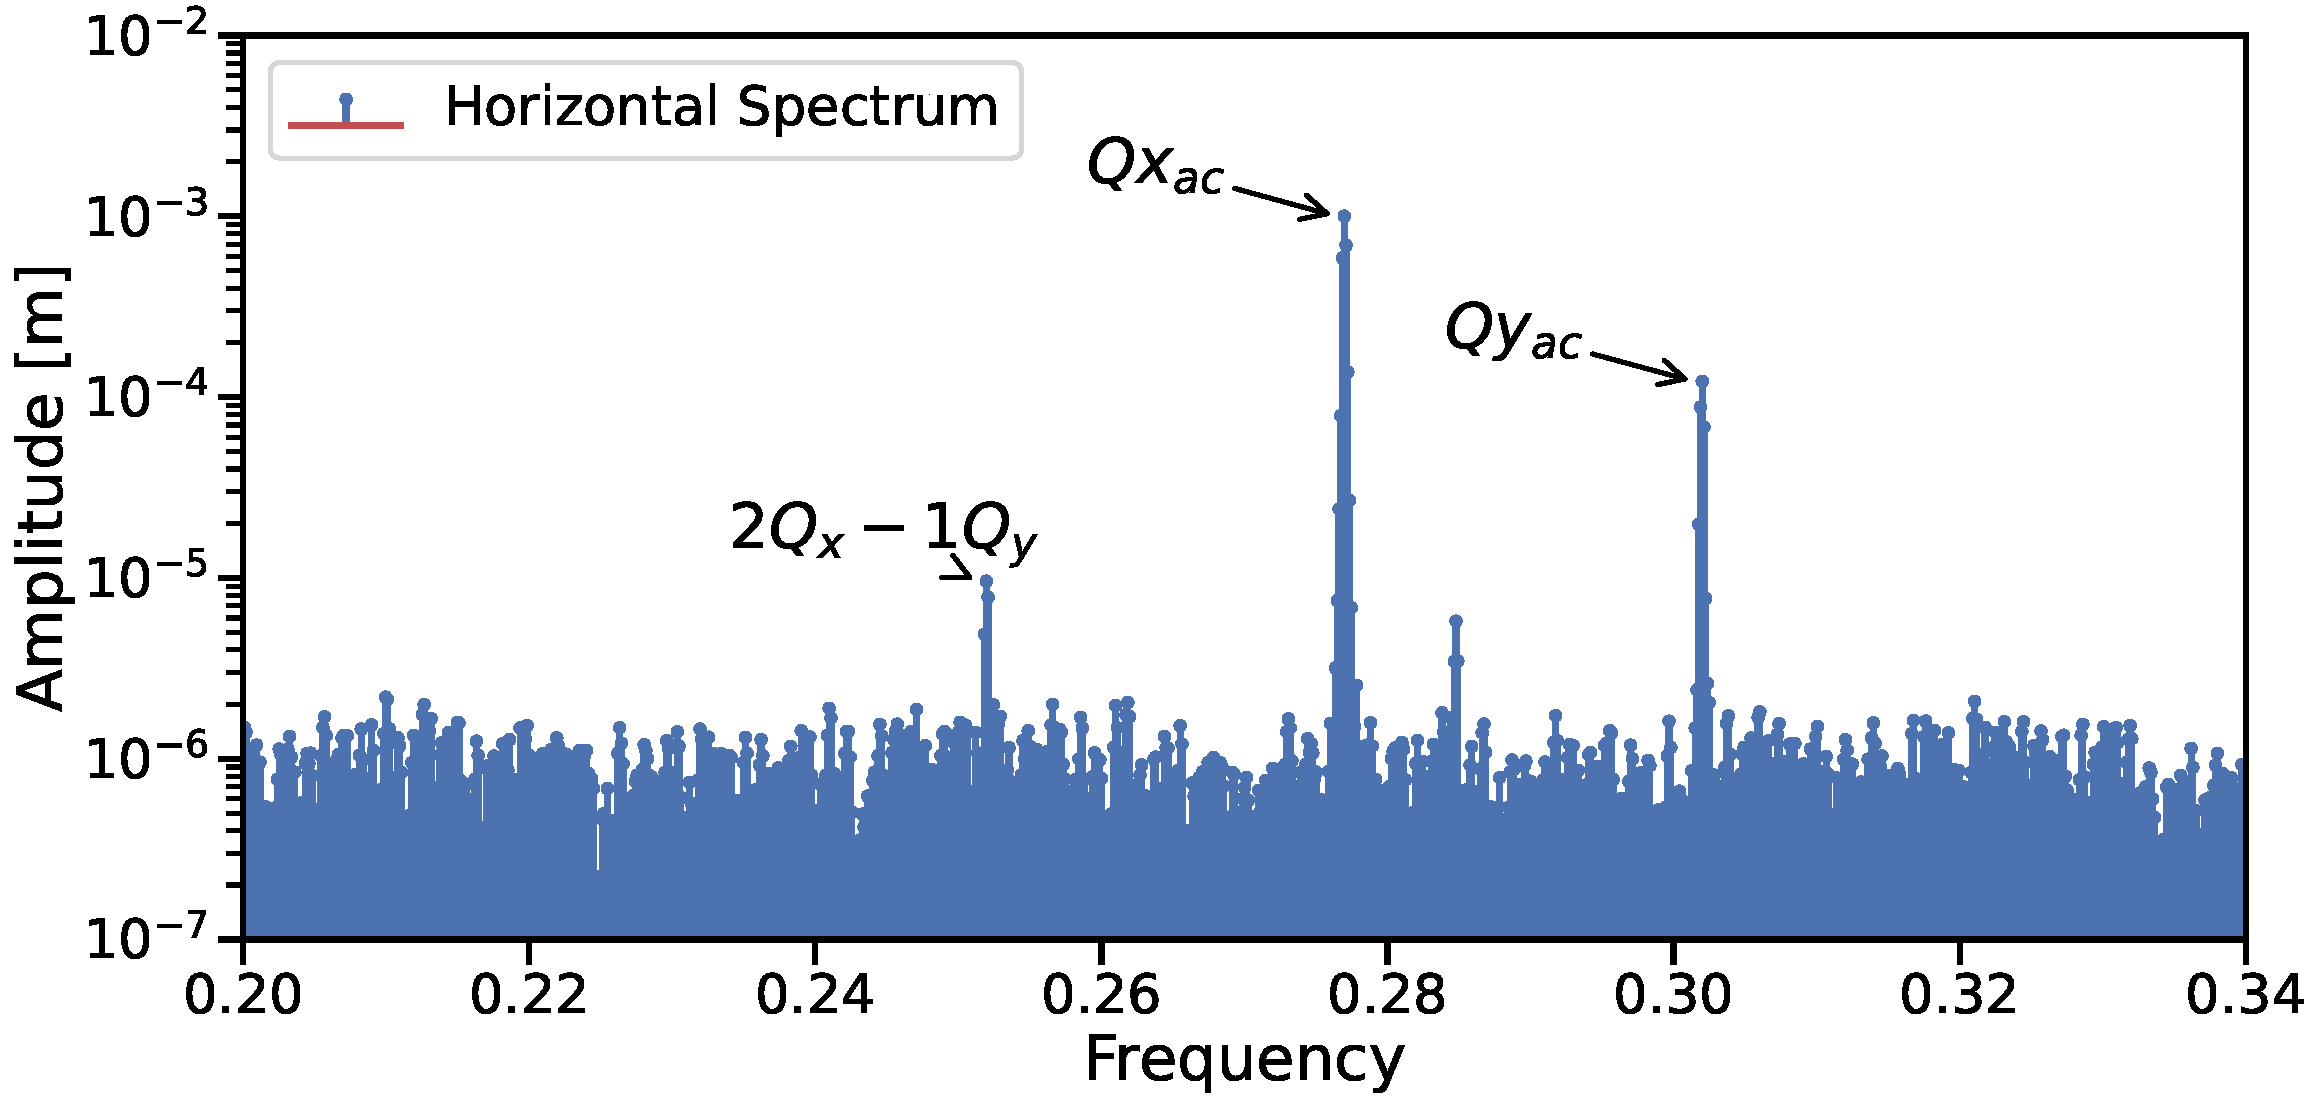
\includegraphics[width=0.8\textwidth]{./images/spectrum_a4_top_energy.pdf}
    \caption{Horizontal spectrum of Beam 1 at top energy before and after application of
    skew-octupolar RDT corrections. The RDT $f_{1210}$ is seen at $2Q_x - 1Q_y$.}
    \label{fig:skew_octupolar:spectrum_a4_top_energy}
\end{figure}




%-----------------------------
%      Response Matrix
%-----------------------------
\subsection{\review{Response Matrix and Corrections}}

To create a response matrix, simulations were conducted with the tunes and AC-Dipole deltas set to
those used for measurements. The natural tunes are $Q_x = 0.285$ and $Q_y = 0.292$ while the driven
tunes are $Q_{x,ac} = Q_x -0.008$ and $Q_{y,ac} = Q_y + 0.01$. Each corrector is then powered
individually for each tracking simulation. As measurements near the IP can be quite noisy, those are
not utilized in the calculation of the correction. The polar plot of
\Cref{fig:skew_octupolar:response_correctors_polar} illustrates the response of each corrector at a
given BPM and can be used to get an intuition of the effect of the correctors.

\begin{figure}[!htb]
    \centering
    \begin{subfigure}{0.7\textwidth}
        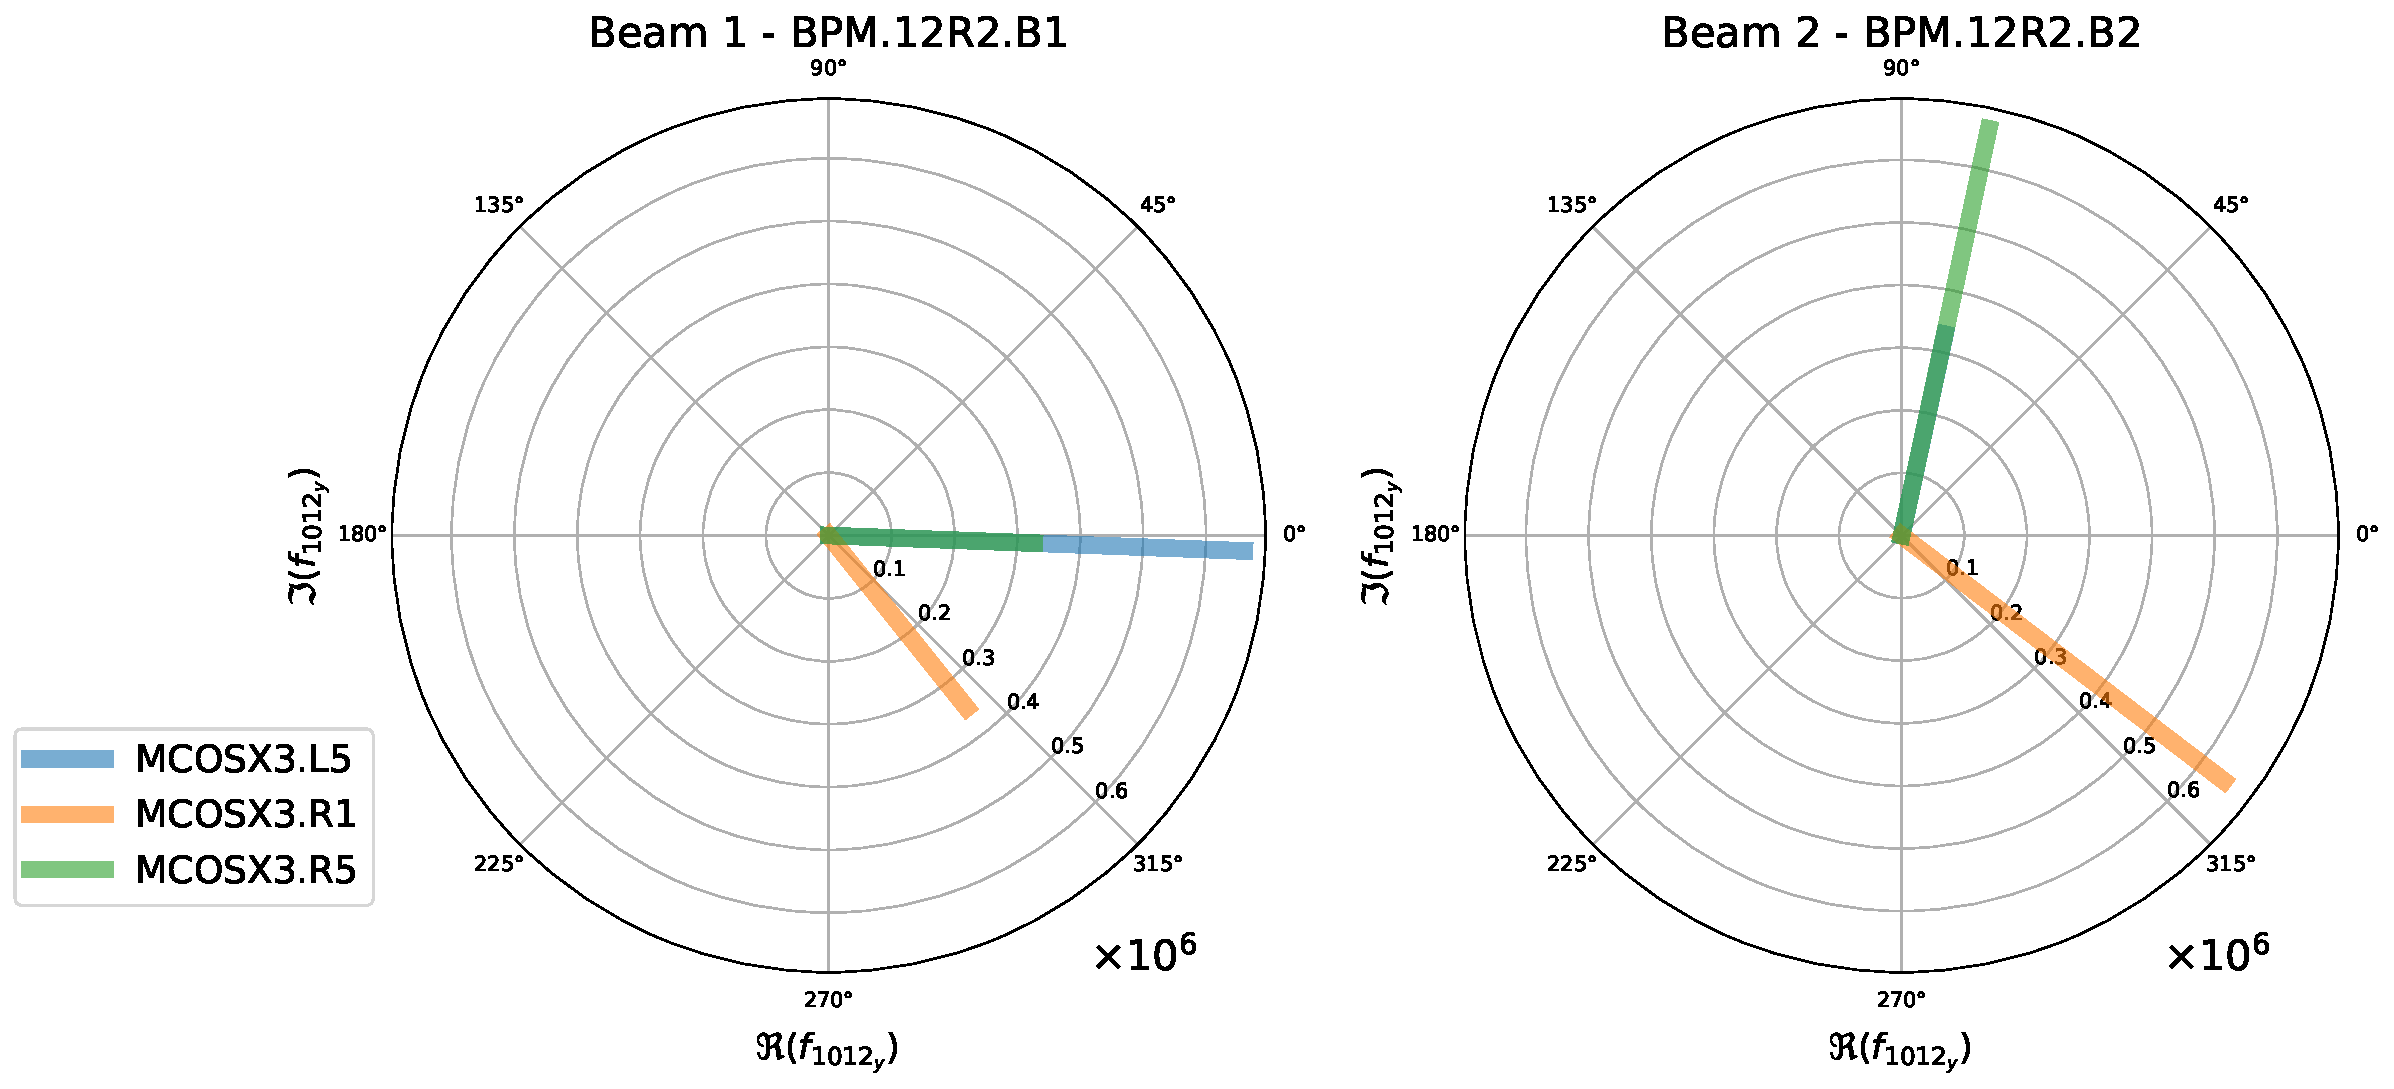
\includegraphics[width=\textwidth]{./images/orthogonal_a4_inj_f1012_y.pdf}
        \caption{$f_{1012,y}$}
    \end{subfigure}
    \par\bigskip 
    \begin{subfigure}{0.7\textwidth}
        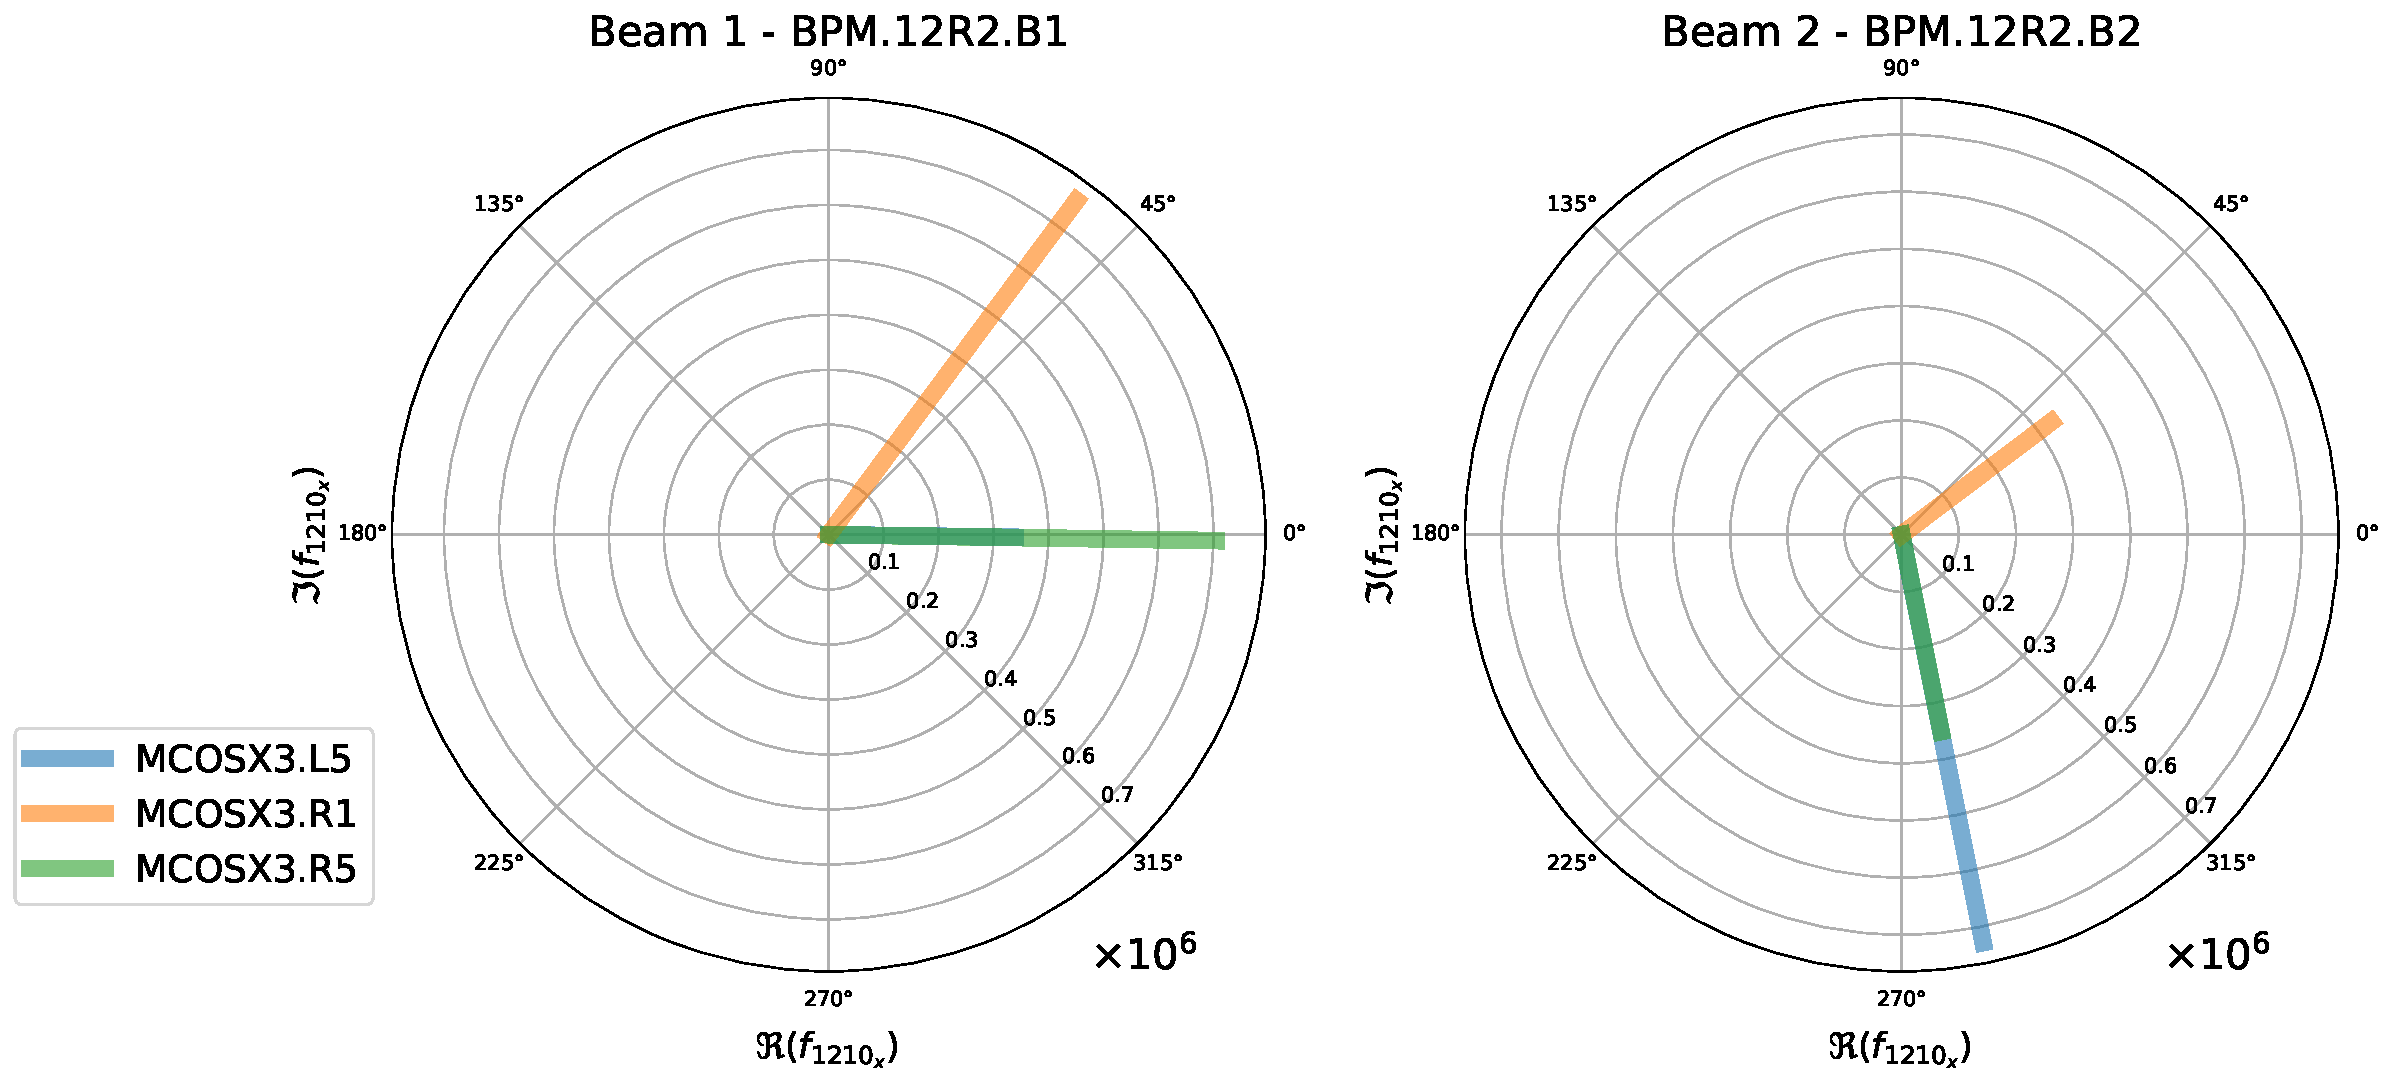
\includegraphics[width=\textwidth]{./images/orthogonal_a4_inj_f1210_x.pdf}
        \caption{$f_{1210,x}$}
    \end{subfigure}
    \caption{Simulated RDTs response of the available skew octupolar correctors at top energy.  Each
    corrector is powered at $J_4 = 1 [\text{m}^{-4}]$. The orthogonality of R1 and L5/R5 allows to
    independently control the real and imaginary parts.}
    \label{fig:skew_octupolar:response_correctors_polar}
\end{figure}

Correctors L5 and R5 having the same angle indicates that either can be used for corrections. Effectively
having only two correctors with different angles, it makes computing corrections for four RDTs (two
per beam) very challenging.  In this context, a response matrix based approach is most effective in
determining the optimal combination of corrector strengths.
\Cref{fig:skew_octupolar:response_correctors} shows the real part of the RDTs from these
simulations for Beam 1. Beam 2 shows a similar level of response for these correctors.

\begin{figure}[!htb]
    \centering
    \begin{subfigure}{0.8\textwidth}
        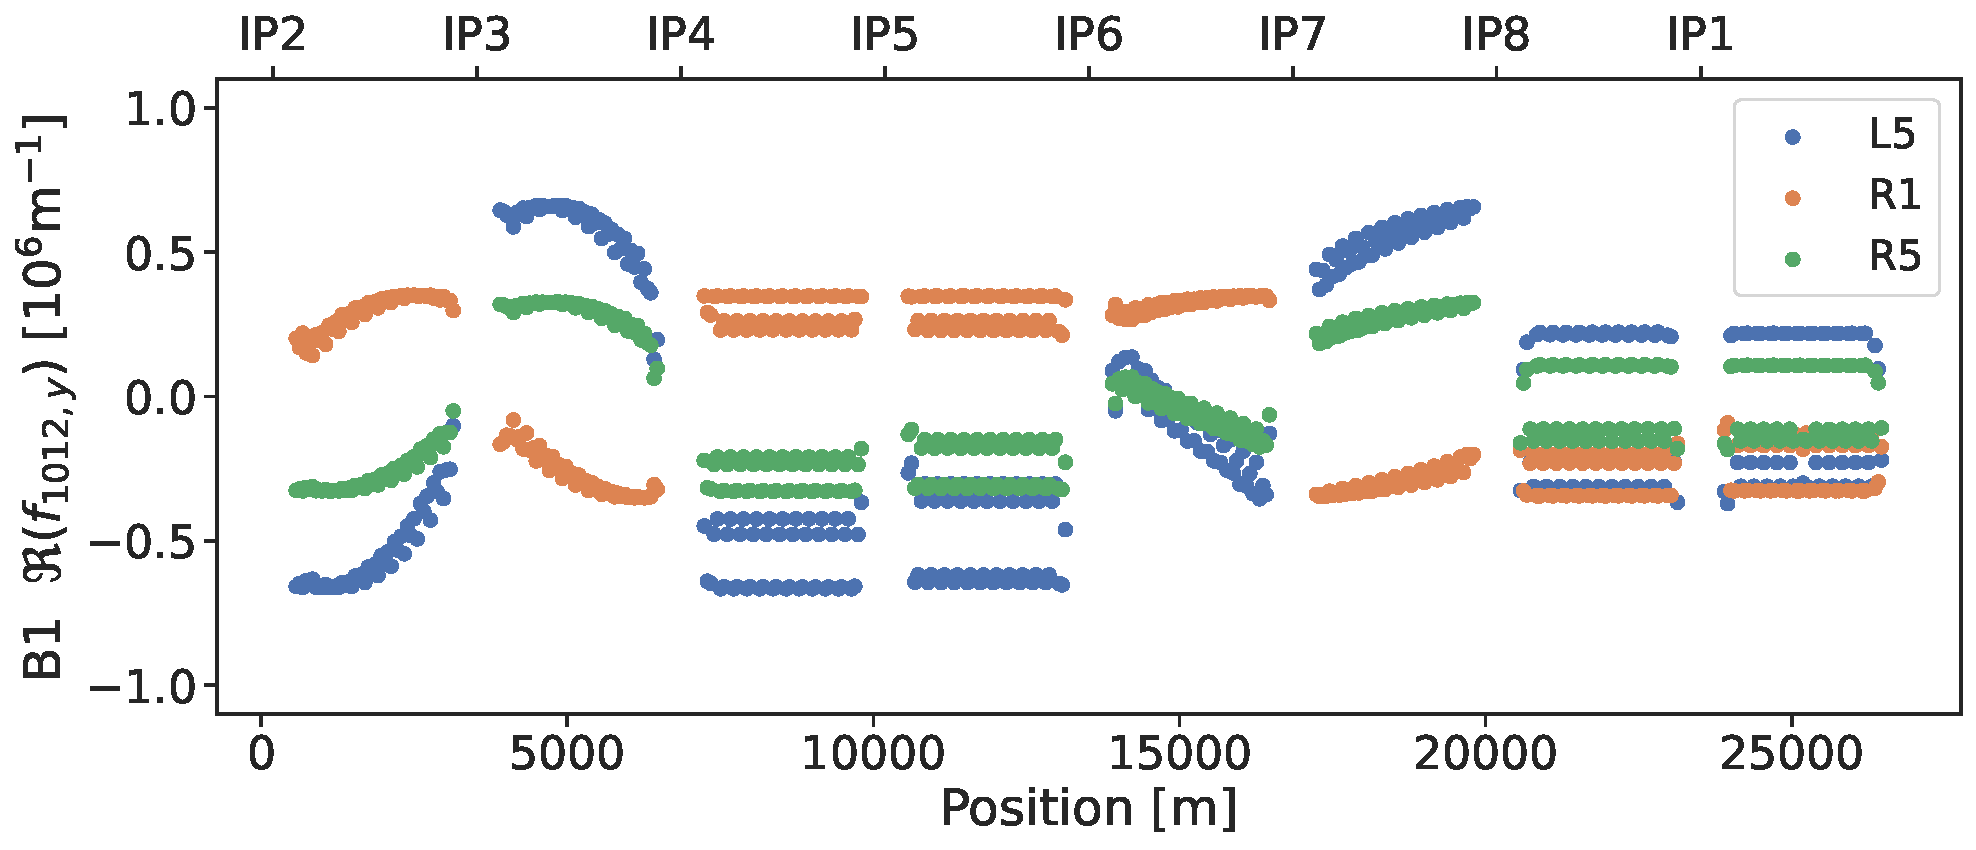
\includegraphics[width=\textwidth]{./images/f1012_b1_correctors.pdf}
        \caption{$f_{1012,y}$}
    \end{subfigure}
    \par\bigskip 
    \begin{subfigure}{0.8\textwidth}
        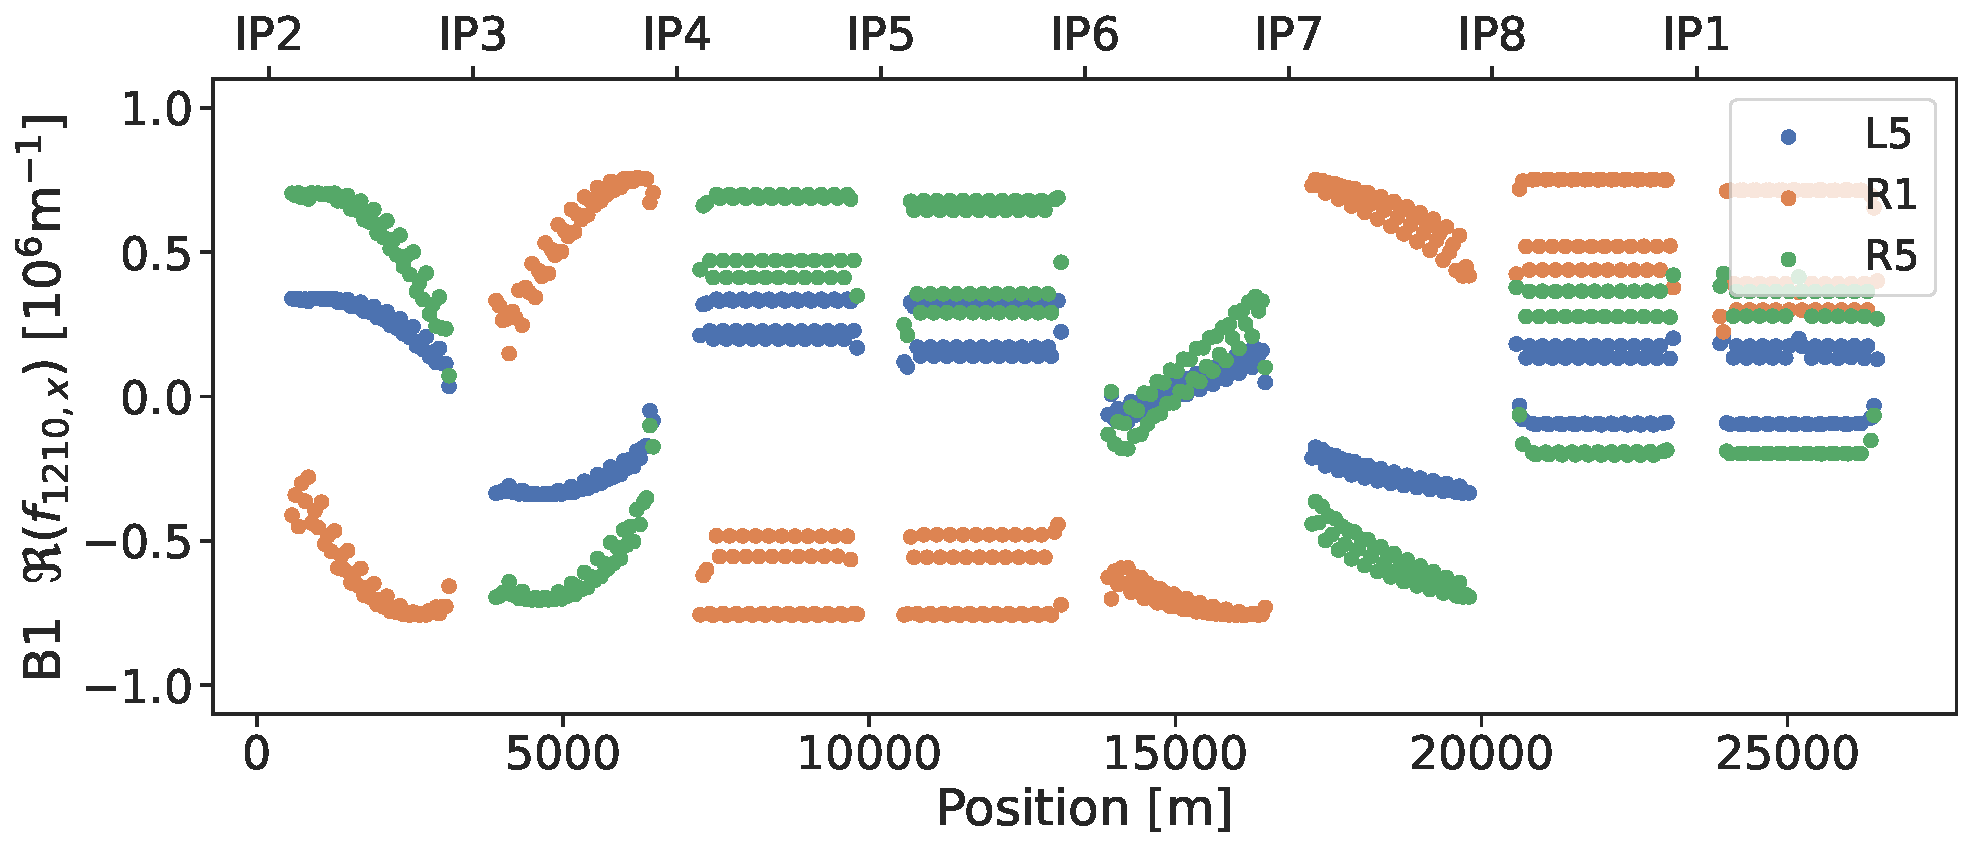
\includegraphics[width=\textwidth]{./images/f1210_b1_correctors.pdf}
        \caption{$f_{1210,x}$}
    \end{subfigure}
    \caption{Simulation of the RDT response of the skew octupolar correctors at top energy for Beam
    1. Each corrector is powered at $J_4 = 1 [\text{m}^{-4}]$.}
    \label{fig:skew_octupolar:response_correctors}
\end{figure}

%%%%

Previous simulations with each corrector powered on are compiled into a matrix, as detailed in
\cref{correction_principle:response_matrix}, to capture the RDT response. By inverting this
matrix, the appropriate set of correctors needed to replicate the measurement is determined.
Finally, multiplying by $-1$ allows for the computation of the required strengths for the set of
correctors. These corrector strengths, for the measured RDTs, are presented in
\cref{tab:skew_octupolar:correction_strengths}.

These corrections have proven to be effective in reducing the RDT amplitudes and have been applied
during 2023's commissioning and later on kept for regular operation. The RDT levels of the bare
machine measured previously and with these corrections are shown in
\cref{fig:skew_octupolar:corrections_vs_bare}. It can be observed that both RDT amplitudes are
reduced, with the exception of $f_{1210,x}$ for Beam 2, which stays constant, while being at an
already low level. The reduction of RDT amplitude is comparable to those obtained in 2018, where the
same RDT for Beam 2 did neither improve or worsen.


\begin{table}[!htb]
    \centering
    \begin{tabular}{lr}
      \toprule
      Corrector    &    Strength $[\text{m}^{-4}]$ \\
      \midrule
      MCOSX3.L1    &           broken  \\
      MCOSX3.R1    &           $-0.50$ \\
      MCOSX3.L5    &           $ 0.42$ \\
      MCOSX3.R5    &           $-0.01$ \\
      \bottomrule
    \end{tabular}
    \caption{Computed corrections for skew octupolar RDTs at top energy. The corrector L1 has been 
    broken for several years and can not be used.}
    \label{tab:skew_octupolar:correction_strengths}
\end{table}
 
\begin{figure}[!htb]
    \centering
    \begin{subfigure}{0.47\textwidth}
        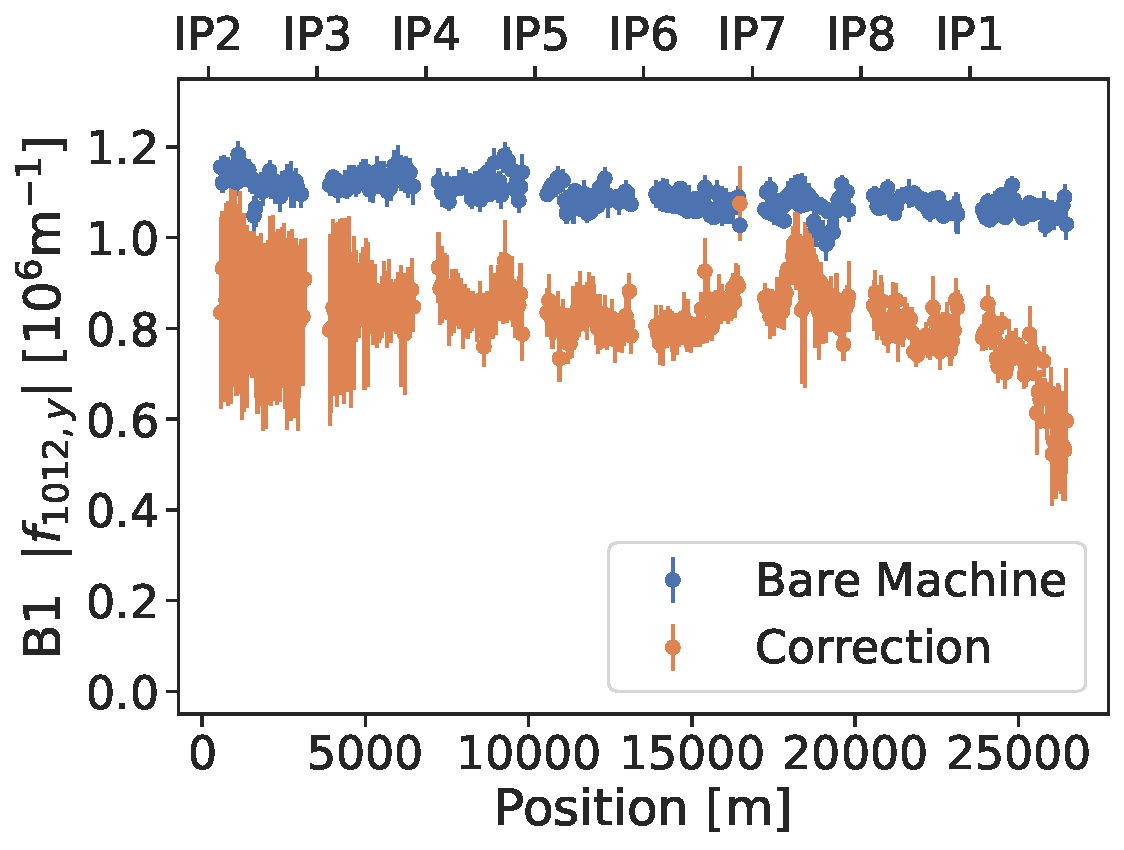
\includegraphics[width=\textwidth]{./images/f1012_b1.pdf}
        \caption{$f_{1012,y}$ Beam 1}
    \end{subfigure}
    \hfill
    \begin{subfigure}{0.47\textwidth}
        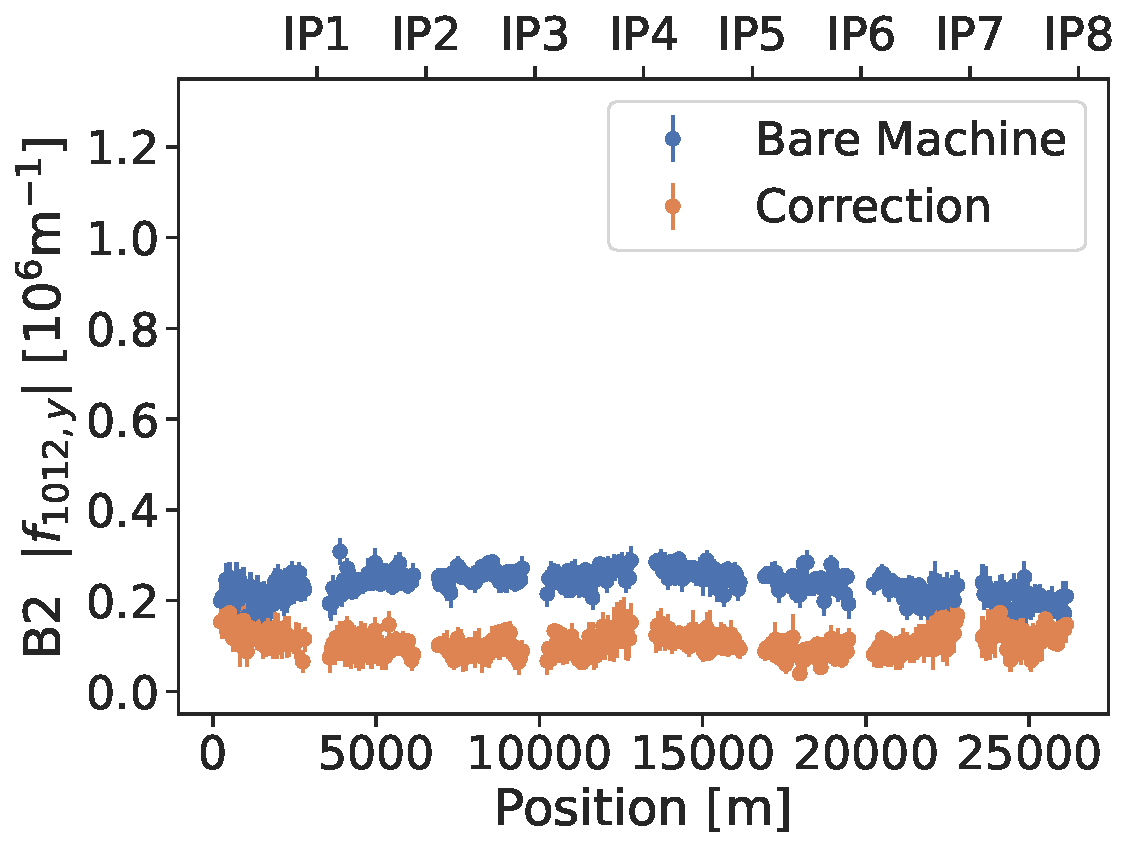
\includegraphics[width=\textwidth]{./images/f1012_b2.pdf}
        \caption{$f_{1012,y}$ Beam 2}
    \end{subfigure}
    %
    \par\bigskip 
    % 
    \begin{subfigure}{0.47\textwidth}
        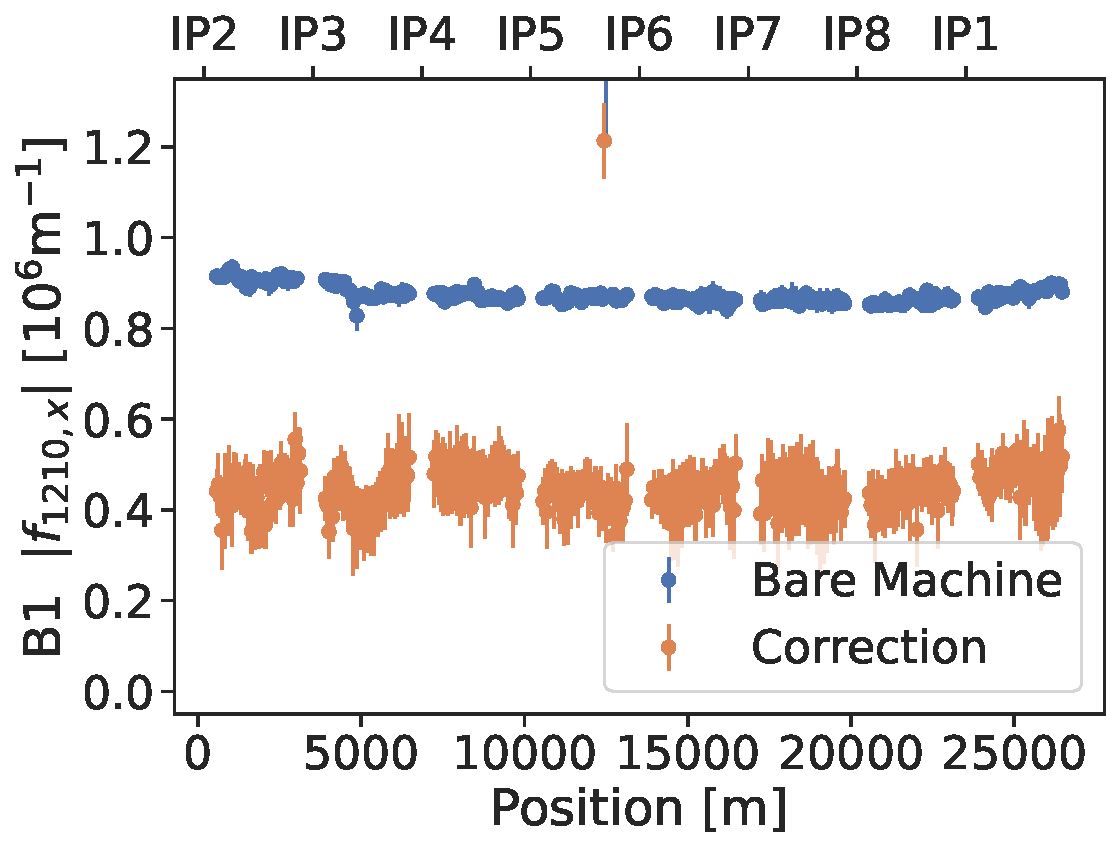
\includegraphics[width=\textwidth]{./images/f1210_b1.pdf}
        \caption{$f_{1210,x}$ Beam 1}
    \end{subfigure}
    \hfill
    \begin{subfigure}{0.47\textwidth}
        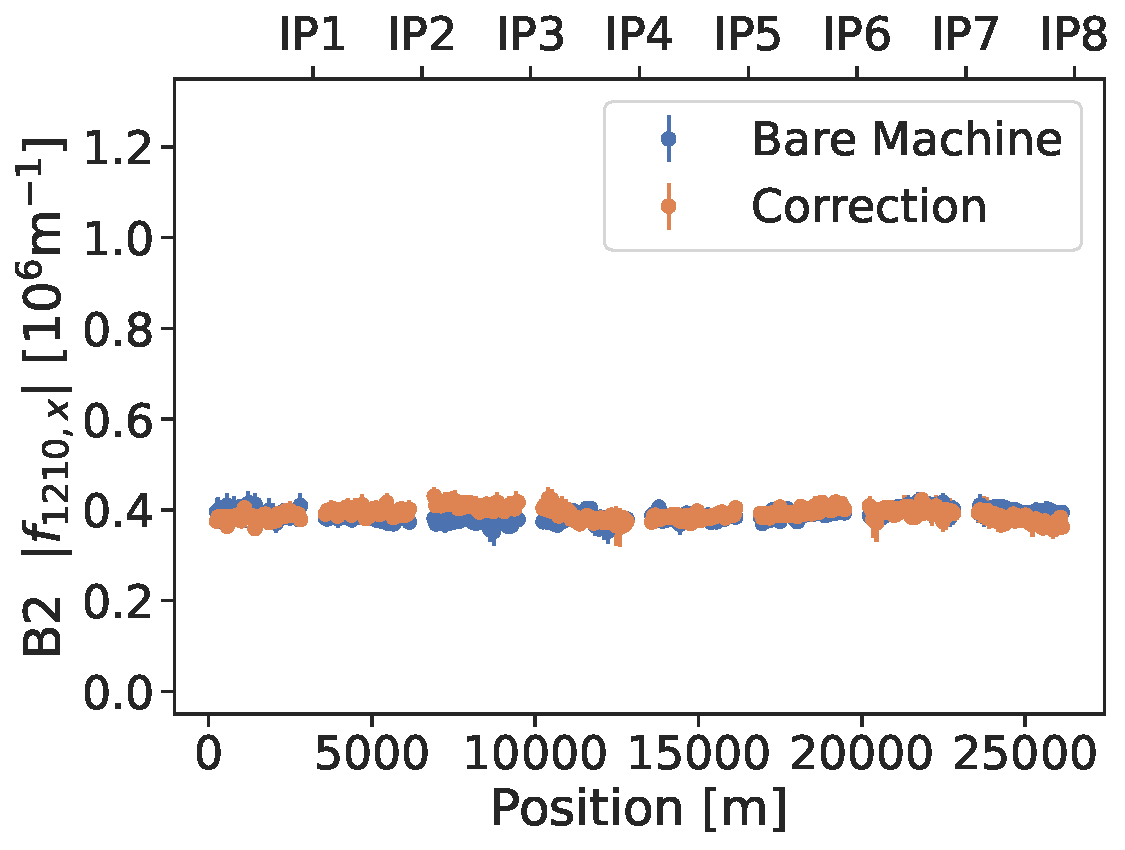
\includegraphics[width=\textwidth]{./images/f1210_b2.pdf}
        \caption{$f_{1210,x}$ Beam 2}
    \end{subfigure}
    \caption{Measured skew octupolar RDTs at top energy and $\beta^*=30\text{cm}$ before and after
    correction. A reduction if observed for all but one RDT in Beam 2.} 
    \label{fig:skew_octupolar:corrections_vs_bare}
\end{figure}

A improvement in the forced dynamic aperture during AC-Dipole excitation was observed with the
earlier skew-octupolar RDTs corrections implemented. \Cref{fig:decapoles:losses_a4_corrs_timeline}
shows the timeline of the various kicks amplitudes before and after corections.
It can clearly seen that skew-octupolar corrections enhance the forced dynamic aperture and allow
for higher-amplitude kicks with the same amount of losses.
%\Cref{fig:decapoles:losses_a4_corrs} illustrates the relative losses when kicking at different
%amplitudes with the AC-Dipole.

\begin{figure}[!htb]
    \centering
    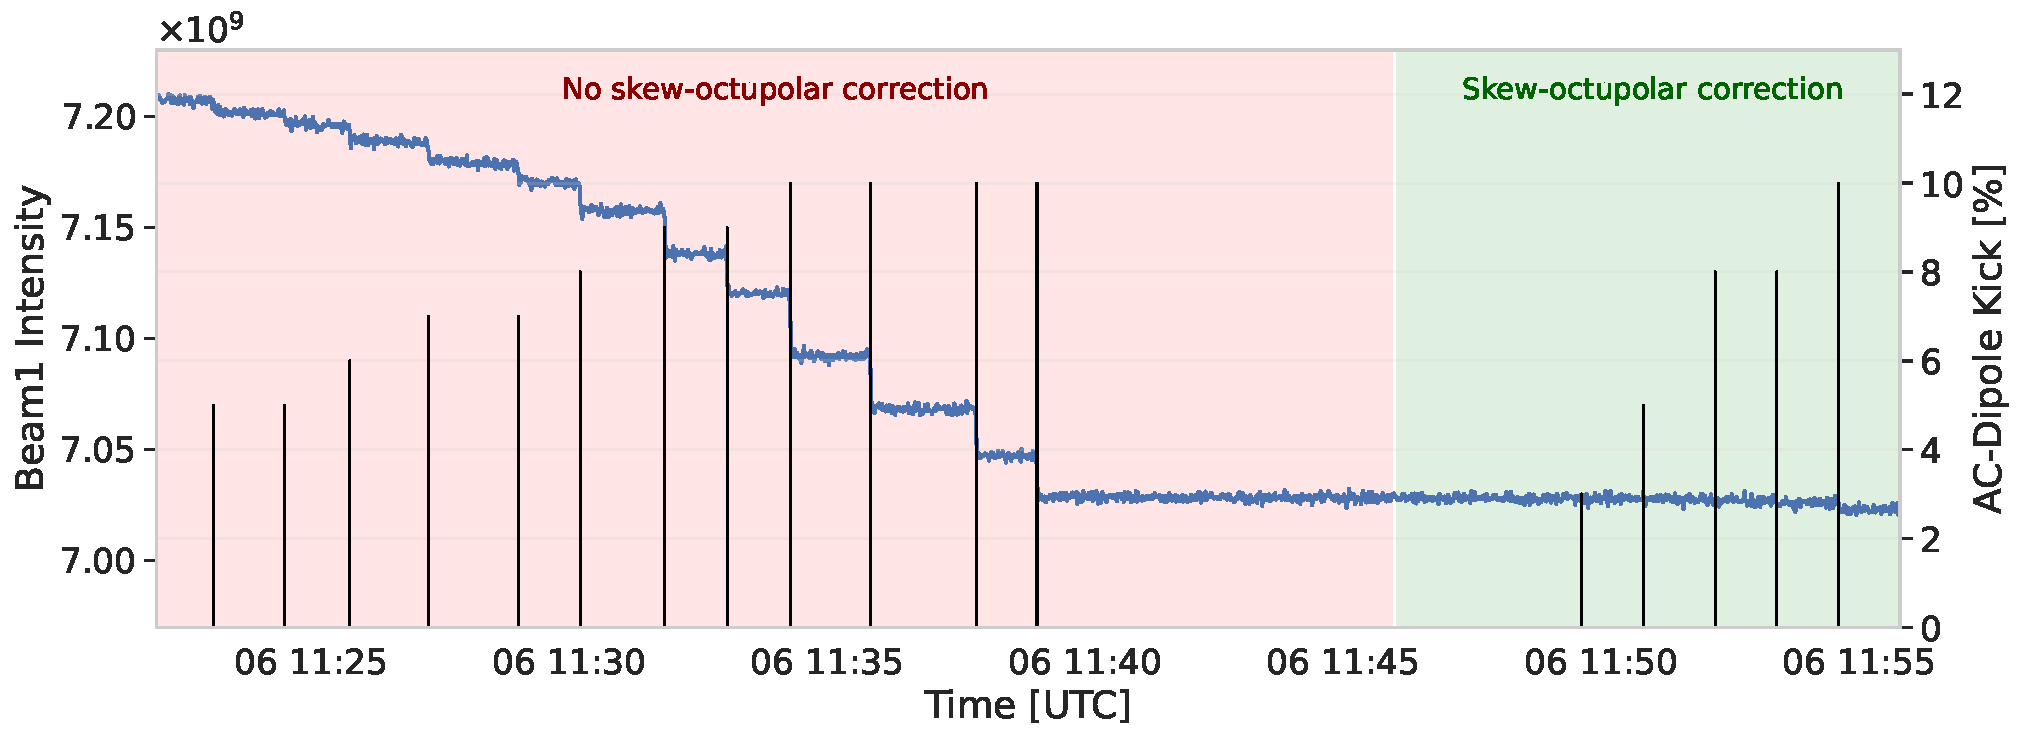
\includegraphics[width=1\textwidth]{./images/timeline_losses_with_without_a4corr.pdf}
    \caption{Intensity of Beam 1 related to the kick percentage of the AC-Dipole over time, before
    and after having applied skew-octupolar RDT corrections.}
    \label{fig:decapoles:losses_a4_corrs_timeline}
\end{figure}

%\begin{figure}[!htb]
%    \centering
%    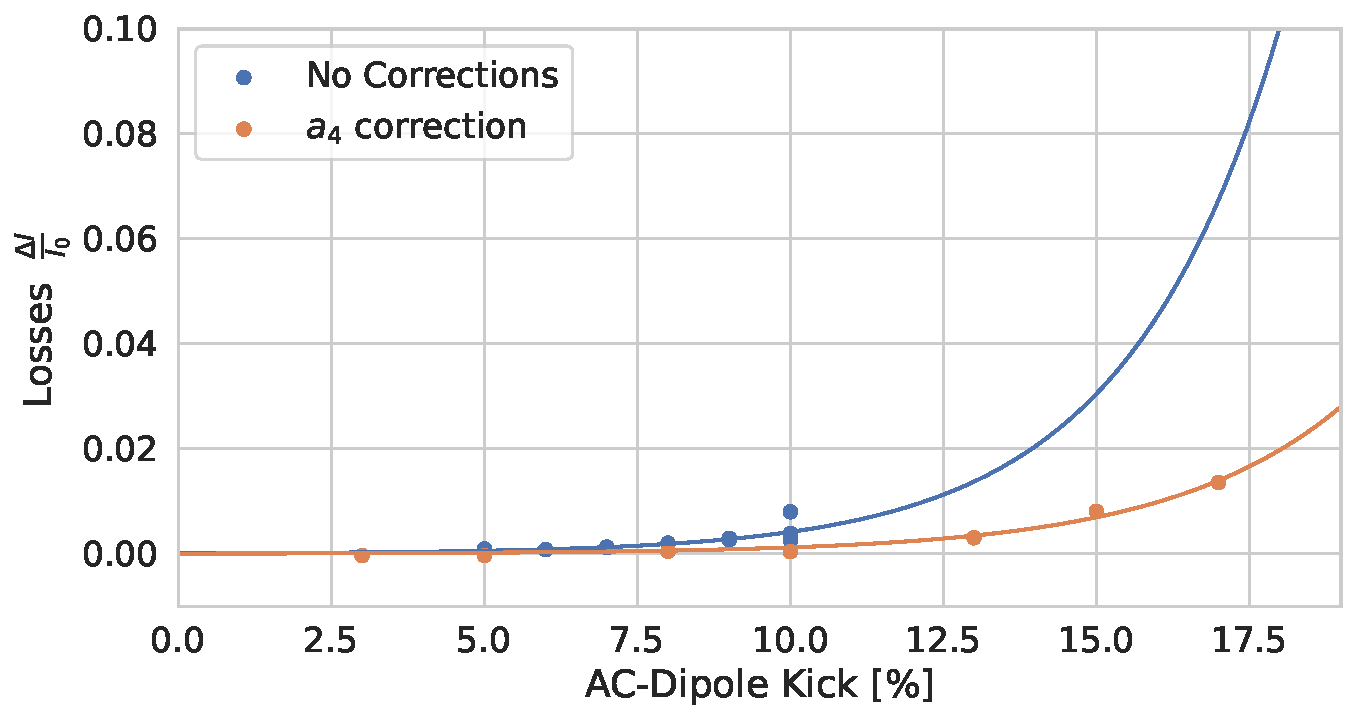
\includegraphics[width=0.8\textwidth]{./images/losses_with_without_a4corr.pdf}
%    \caption{Relative losses experienced with AC-Dipole kick amplitude with and without corrections
%    pertaining to skew-octupolar RDTs $f_{1012}$ and $f_{1210}$.}
%    \label{fig:decapoles:losses_a4_corrs}
%\end{figure}


Skew-octupolar Resonance Driving Terms have, for the first time, been directly corrected using a
response matrix-based approach at top energy. This new approach allows for a more efficient
use of dedicated machine time compared to the previous empirical approach. Corrections have
significantly improved the forced dynamic aperture, enabling the high amplitude kicks necessary for
non-linear optics measurements.
Furthermore, these corrections can be computed online in the control room, reducing commissioning
time and thereby increasing the integrated luminosity of the LHC.




%=============================
%    Landau Contribution
%=============================
% https://indico.cern.ch/event/1351567/contributions/5708754/attachments/2773145/4832599/2023-12-15_MO_Roll_Coupling_complete.pdf
\FloatBarrier
\section{\review{Skew-Octupolar RDT driven by Landau Octupoles}}


%-----------------------------
%        Introduction
%-----------------------------
%\subsection{\review{Introduction}}

The significant progress achieved in understanding skew octupolar RDTs at top energy and their
corrections improving the forced dynamic aperture prompted their study at injection energy, where they had
never been studied before. During these studies, large skew octupolar resonances lines were observed
when Landau octupoles were powered. These magnets, being normal octupoles, are not expected to
contribute to skew octupolar fields. To further understand and characterize the contribution of
Landau octupoles to skew octupolar fields, subsequent measurements were conducted. Measurements of
the RDTs introduced in \cref{tab:skew_octupolar:resonances_rdts}, were performed with several
strengths of Landau octupoles, ranging from $-2 K_4$ to $5 K_4$.

The following \cref{fig:skew_octupolar:mo_different_levels_meas} illustrates the measured amplitude
for Beam 1 of the RDT $f_{1210}$ with these varying strengths of Landau octupoles. It can be
observed that normal octupoles have a large impact on this RDT at only $K_4 = 5$. This amplitude is
expected to increase by an order of magnitude with the nominal powering of Landau octupoles at
$K_4 = 18$ and significantly supports the need for their study.

%All measurements were taken at injection energy at tunes of $Q_x = 0.275$, $Q_y = 0.293$ and
%AC-Dipole deltas of $\Delta Q_x = -0.01$ and $\Delta Q_y = -0.011$. Although both beams were
%measured, this section focuses on Beam 1 to preliminarily investigate the matter.

\begin{figure}[!htb]
    \centering
    \begin{subfigure}{0.8\textwidth}
        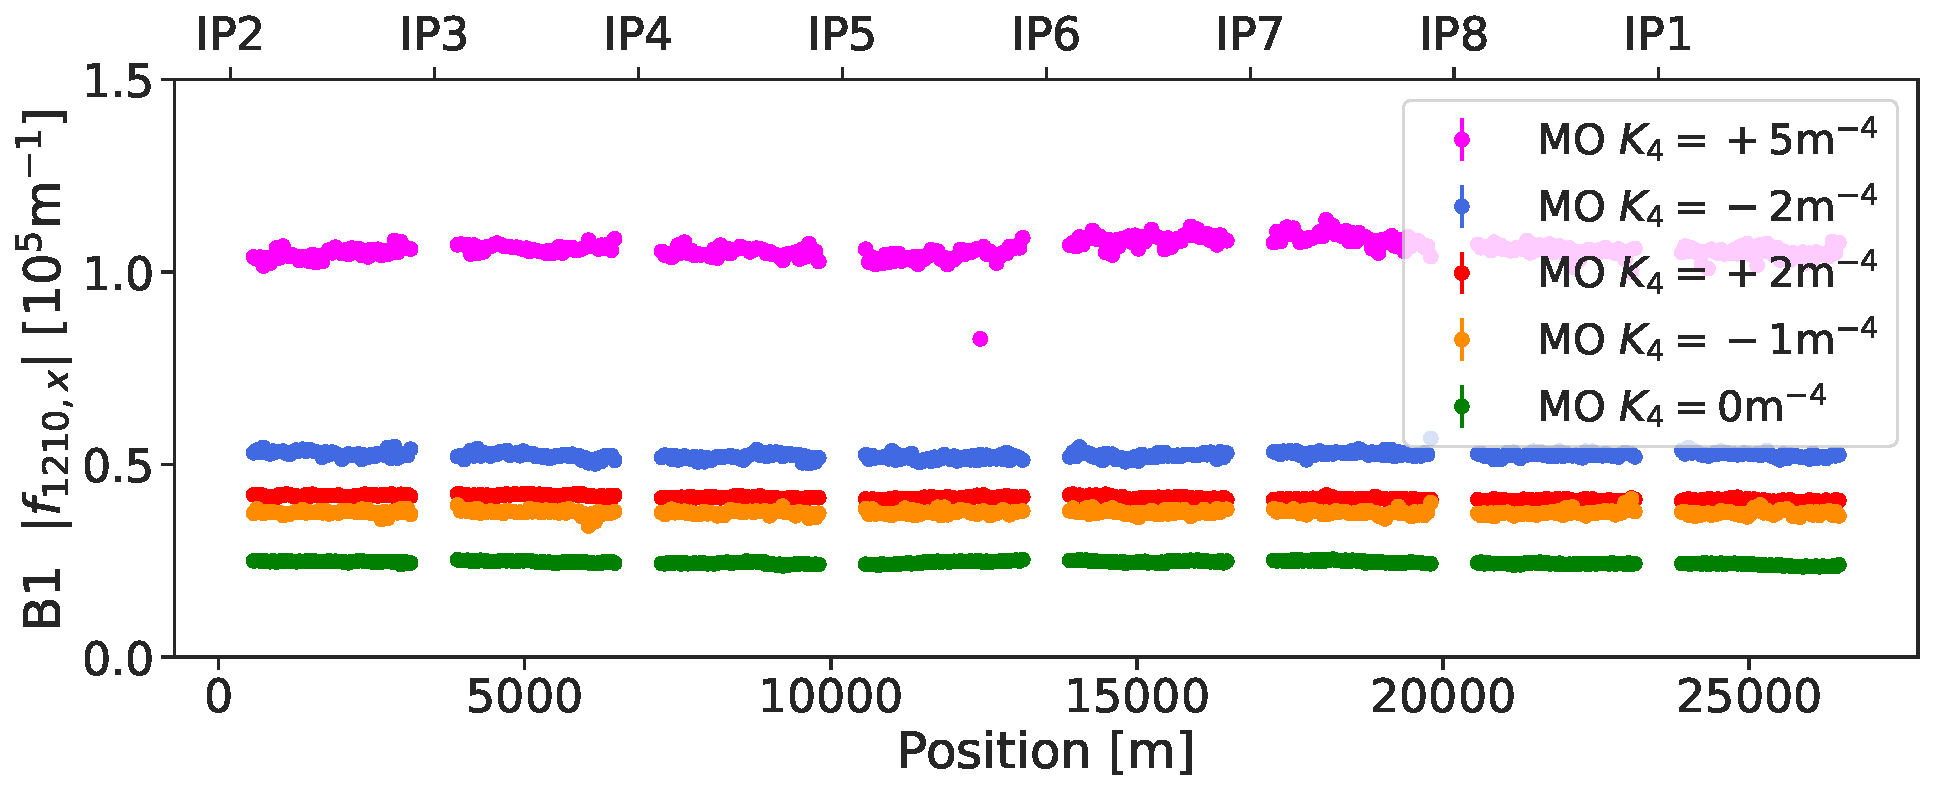
\includegraphics[width=\textwidth]{./images/skew_octupoles/f1210_AMP_all_measurements.pdf}
    \end{subfigure}
    \caption{Unexpected amplitude shift of skew-octupolar RDT $f_{1210}$ with varying Landau
    octupoles strengths.}
    \label{fig:skew_octupolar:mo_different_levels_meas}
\end{figure}

Simulations conducted with Landau powering of $K_4 = 0$ and $K_4 = 2$, incorporating additional
normal and skew field errors, do not replicate the measured shift. The comparison between
measurements and simulations is presented in \cref{fig:skew_octupolar:mo_meas_vs_sim_+2}, where it
is evident that some component is absent from the magnetic model. For conciseness, all figures are
shown with respect to Beam 1, although similar results are observed for Beam 2.

\begin{figure}[!htb]
    \centering
    \begin{subfigure}{0.8\textwidth}
        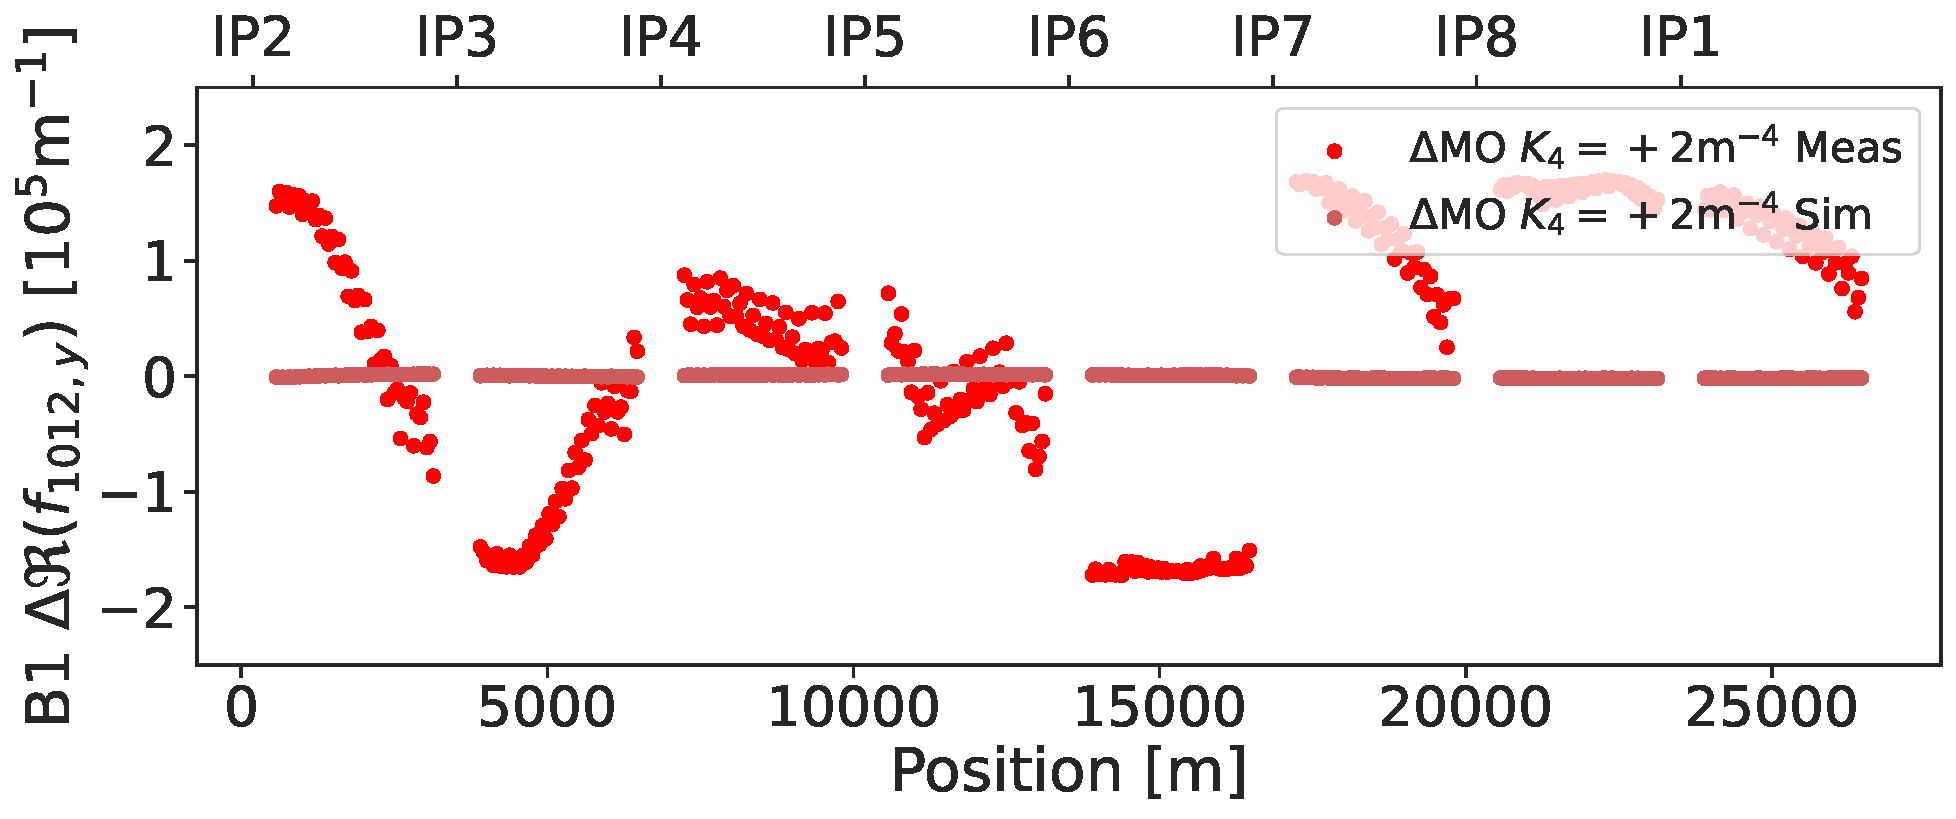
\includegraphics[width=\textwidth]{./images/skew_octupoles/f1012_meas_vs_sim_0shift.pdf}
        %\caption{$f_{1012,y}$}
    \end{subfigure}
    \caption{Measured and simulated shift of skew-octupolar RDT after increase of Landau octupoles
    strength from zero. It is apparent that the shift in measurement is not replicated by the
    simulation.}
    \label{fig:skew_octupolar:mo_meas_vs_sim_+2}
\end{figure}



%-----------------------------
%        Misalignments
%-----------------------------
\FloatBarrier
\subsection{\review{Misalignments}}

Magnet misalignments in the LHC have been previously measured and corrected in several
phases~\cite{missiaen_final_2008}. Nevertheless, residual misalignments persist and have been
incorporated into the tables used for simulations. These misalignments include horizontal and
vertical errors, as well as roll errors. While translation errors may induce feed-down effects,
roll errors introduce the skew counterpart of normal magnetic fields, and vice versa.

To assess whether roll errors could explain the behavior observed in measurements, a tracking
simulation was conducted with and without roll errors applied to the Landau octupoles, powered at 
$K_4 = 2$. The amplitude of the RDT $f_{1012}$ is presented in
\cref{fig:skew_octupolar:sim_misalign}, with similar results observed for $f_{1210}$. These
results reveal an imperceptible difference between the two simulations.
Roll errors are unable to account for the previously observed shifts. The average roll error of
the Landau octupoles is indeed small, approximately $0.08$ mrad.

\begin{figure}[!htb]
    \centering
    \begin{subfigure}{0.8\textwidth}
        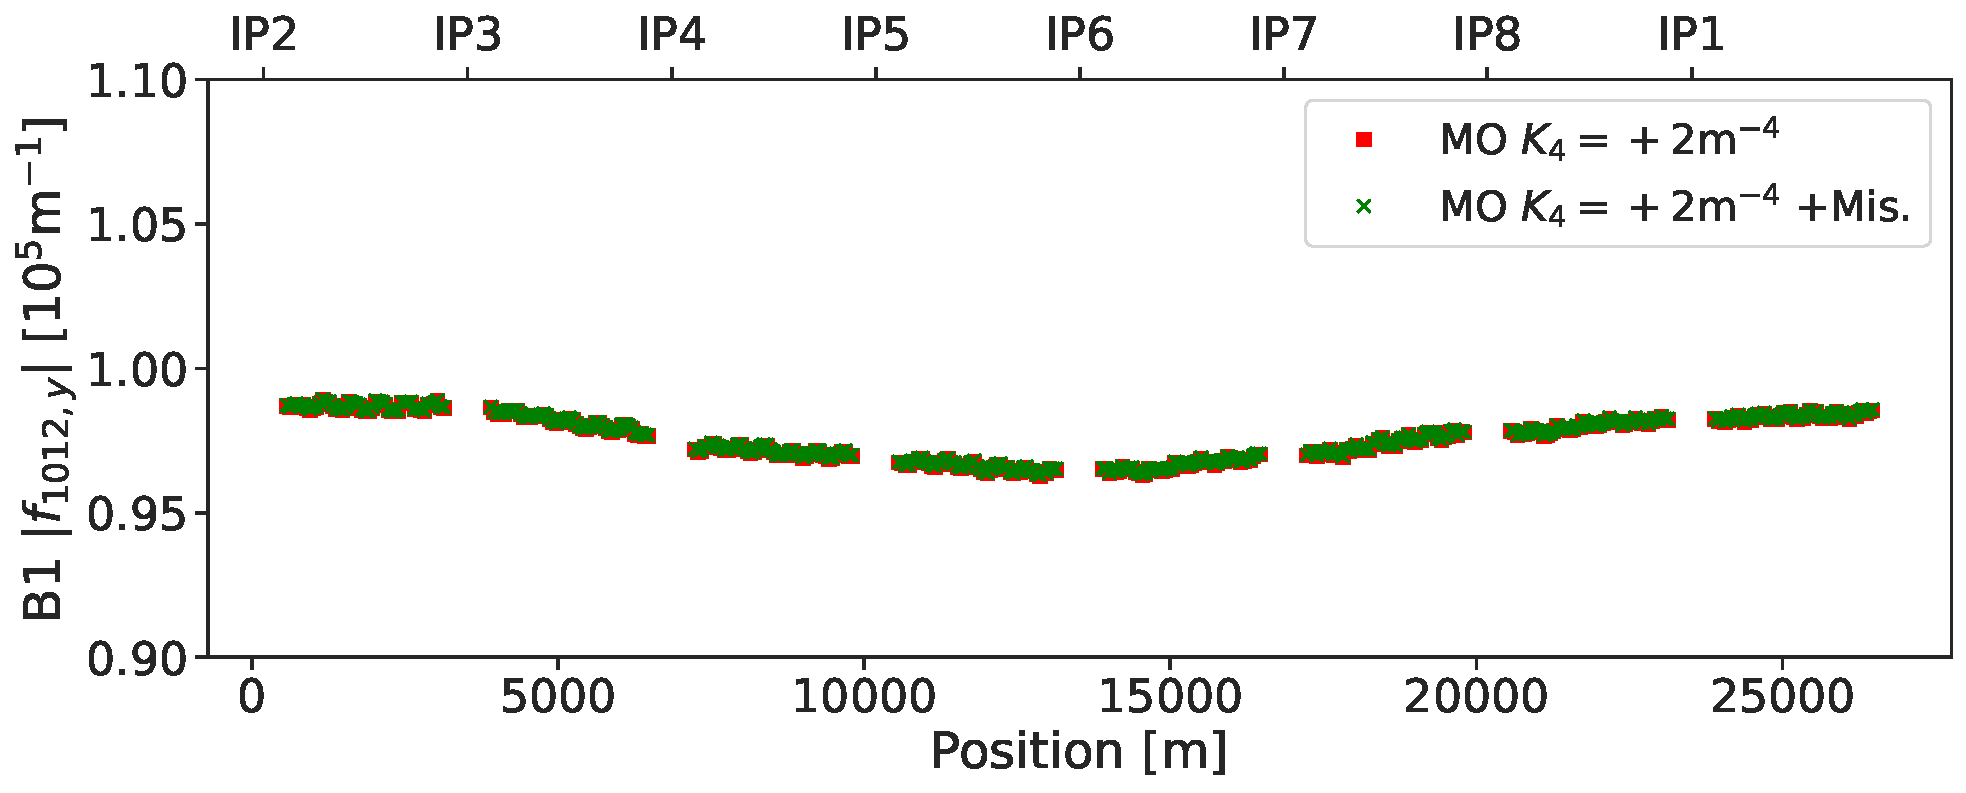
\includegraphics[width=\textwidth]{./images/skew_octupoles/f1012_misalign_AMP.pdf}
        %\caption{$f_{1012,y}$}
    \end{subfigure}
    \caption{Simulated skew octupolar RDT with normal and skew octupolar errors, and Landau
    octupoles powered. One simulation includes further roll errors on the Landau octupoles. No 
    significant difference is observed between the two.} 
    \label{fig:skew_octupolar:sim_misalign}
\end{figure}



%-----------------------------
%        Coupling
%-----------------------------
\FloatBarrier
\subsection{\review{Linear Coupling}}

As misalignments could not explain the discrepancy, it is necessary to consider another source of
errors. According to~\cite{bazzani_normal_1994}, the combination of a normal octupole and a skew
quadrupole can yield skew-octupolar-like fields. Linear coupling can effectively be modeled as a
skew quadrupole and may be a source of the observed discrepancy. The transfer map for an octupole
and a skew quadrupole is detailed in \cref{appendix:transfer_map:skew_quadrupole_and_octupole}.

To test this hypothesis, simulations were initially conducted with varying values of coupling while
maintaining a fixed octupolar strength, allowing for an assessment of the impact of coupling alone.
The resulting RDT $f_{1012}$ is shown in \cref{fig:skew_octupolar:sim_coupling}, with a similar
trend observed for $f_{1210}$. The presented $C^{-}$ values are commonly encountered in
operation and are well within the tolerances established in the LHC design~\cite{bruning_lhc_2004}.
These results indicate that the skew octupolar RDTs are expected to be significantly altered as
coupling increases.


\begin{figure}[!htb]
    \centering
    \begin{subfigure}{0.8\textwidth}
        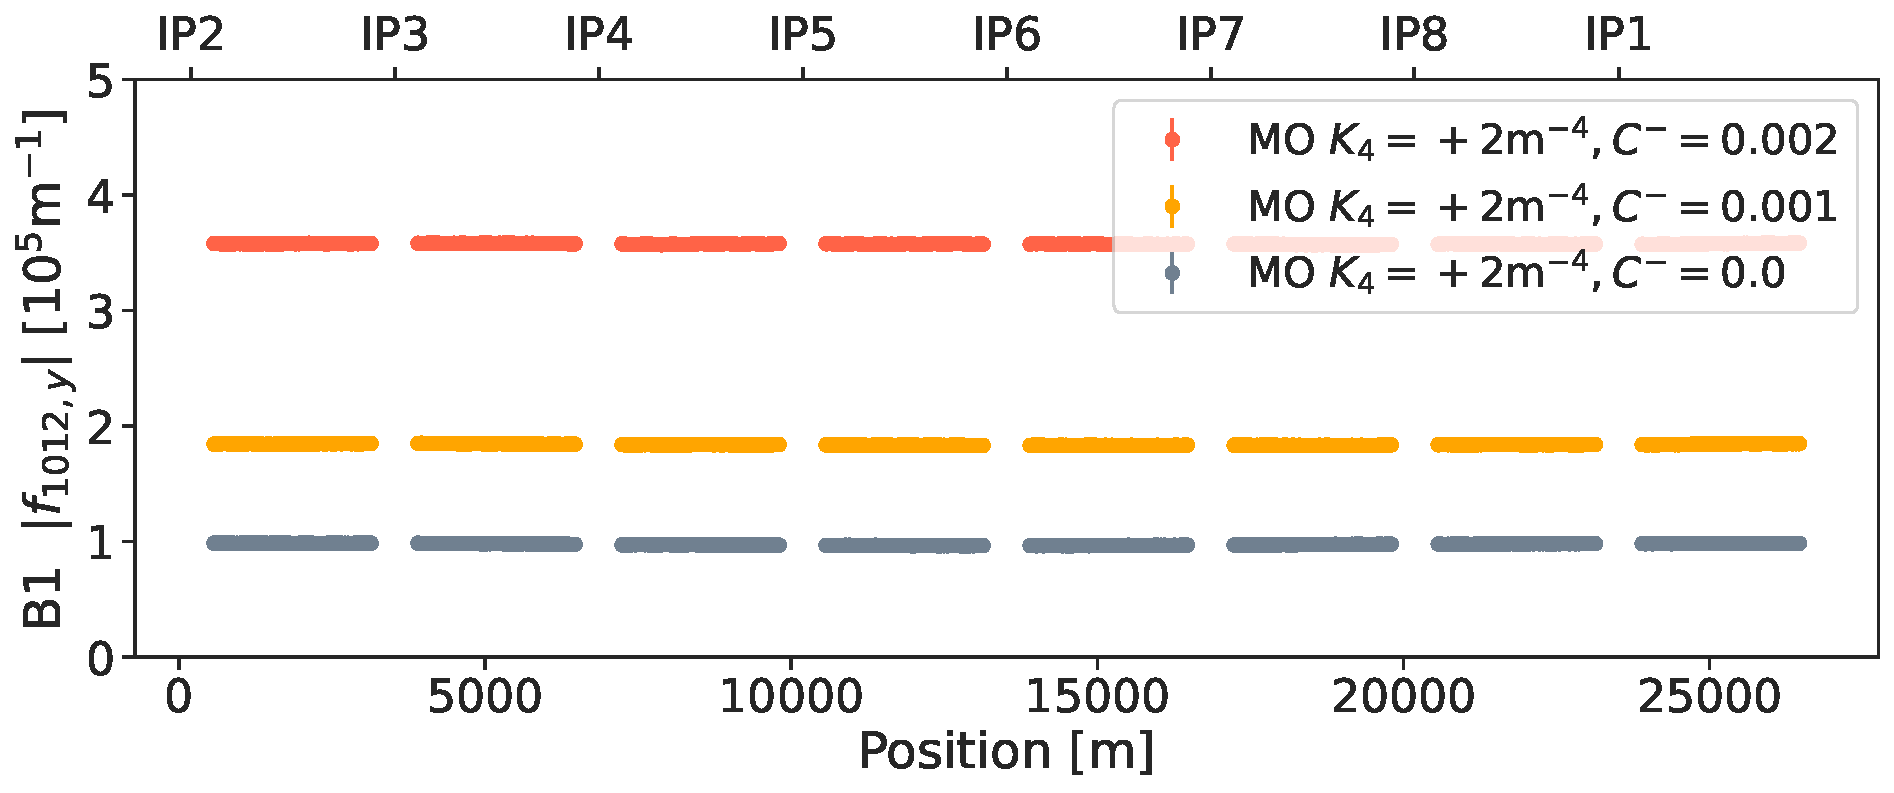
\includegraphics[width=\textwidth]{./images/skew_octupoles/f1012_coupling_sim_AMP.pdf}
    \end{subfigure}
    \caption{Simulated skew octupolar RDT with fixed Landau octupole strength but varying coupling.
    Selected coupling values are often seen in operation.}
    \label{fig:skew_octupolar:sim_coupling}
\end{figure}



%-----------------------------
%          Responses
%\FloatBarrier
%\subsubsection{\review{Responses with Coupling}}

%\begin{table}[!htb]
%    \centering
%    \begin{tabular}{cccc}
%    \toprule
%    &&\multicolumn{2}{c}{Rel. Diff. [\%]} \\
%    \cmidrule{3-4}
%    $K_4$ $[\text{m}^{-4}]$ & RDT & Real & Imag. \\
%    \midrule
%    \multirow{2}{*}{+5}
%     & $f_{1210}$ & 6 & 6  \\
%     & $f_{1012}$ & 12  & 11 \\[0.5em]
%    \multirow{2}{*}{+2}
%     & $f_{1210}$ & 32  & 34  \\
%     & $f_{1012}$ & 36  & 36  \\[0.5em]
%    \multirow{2}{*}{-1}
%     & $f_{1210}$ & 26 & 25 \\
%     & $f_{1012}$ & 21 & 20 \\[0.5em]
%    \multirow{2}{*}{-2}
%     & $f_{1210}$ & 19  & 17  \\
%     & $f_{1012}$ & 21 & 20 \\
%    \bottomrule
%    \end{tabular}
%    \caption{Relative difference between measured and simulated RDT shift induced by the
%    Landau octupoles in presence of coupling. Real parts are illustrated in
%    \cref{fig:skew_octupolar:response_meas_sim_coupling}.}
%    \label{tab:skew_octupolar:rms_ratios}
%\end{table}

Having established that coupling can significantly contribute to the generation of skew octupolar
fields from normal octupoles, further simulations were conducted to match the measured coupling for
each set of observations. Initially, local coupling is assessed using coupling RDTs, followed by the
definition of a set of correctors linked to a common control knob to globally correct the coupling
across the machine. This global knob setting is then applied in simulations to replicate the
measured coupling.
The measured and simulated shifts in the real part of the RDTs $f_{1012}$ and $f_{1210}$, resulting
from the application of various octupole powerings in the presence of coupling, are shown in
\cref{fig:skew_octupolar:response_meas_sim_coupling}. A similar trend is observed for the imaginary
part.
% The relative RMS deviation between simulations and measurements is given
%for each set of strengths and RDTs in \cref{tab:skew_octupolar:rms_ratios}.

It can be observed that simulations and measurements for positive strengths ($K_4=2$ and $K_4=5$) 
are now in good agreement. This suggests that the primary contribution to the skew octupolar RDTs
can be attributed to the Landau octupoles and coupling. The relative deviation between measurement
and simulation can be explained by the sensitivity to the coupling. A difference of $10^{-4}$ units 
is enough to be noticeable, making accurate reproduction of skew octupolar RDTs not trivial.
%
It is to be noted that measurements of $f_{1012}$ with \textit{negative} strength exhibit a
response that is opposite to the predictions made by simulations, whereas $f_{1210}$ agrees well
with the expected results. This behavior may be attributed to magnetic hysteresis. Specifically, the
measurements at positive $K_4$ were taken after a degaussing cycle of the Landau octupoles, while
the negative measurements were conducted immediately afterwards the positive ones. Additional
measurements, with proper degaussing performed before each test, could help clarify this difference.

\begin{figure}[!htb]
    \centering
    \begin{subfigure}{0.47\textwidth}
        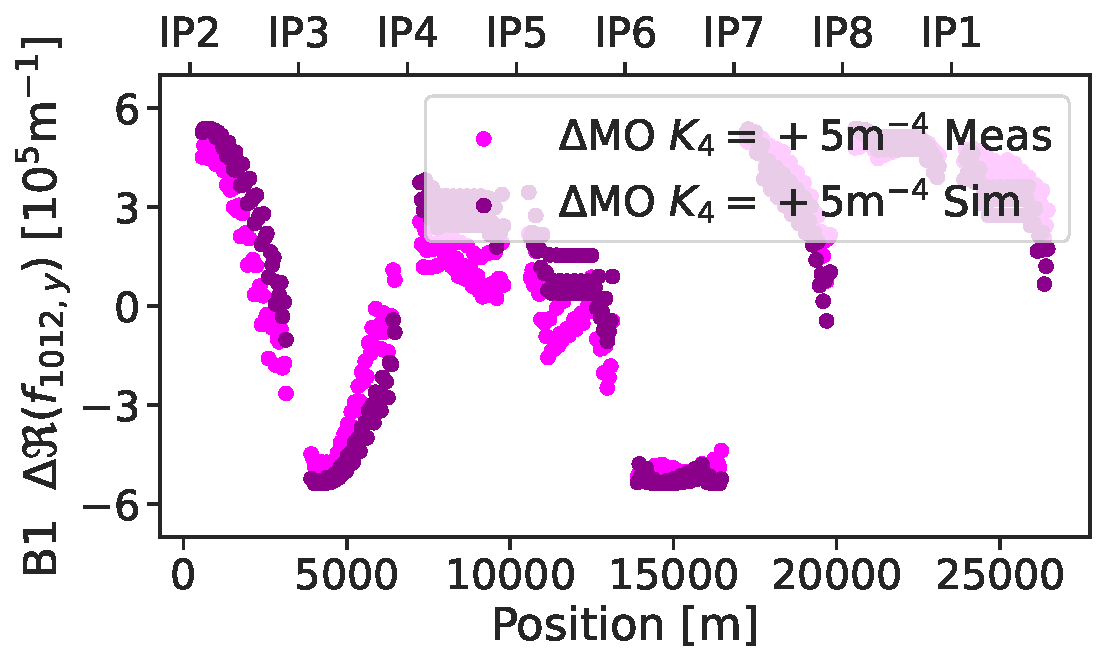
\includegraphics[width=\textwidth]{./images/skew_octupoles/responses_coupling/f1012_response_meas_sim_+5_REAL_smoll.pdf}
        %\caption{$f_{1012,y}$ for $K_4 = +5$}
    \end{subfigure}
    \hfill
    \begin{subfigure}{0.47\textwidth}
        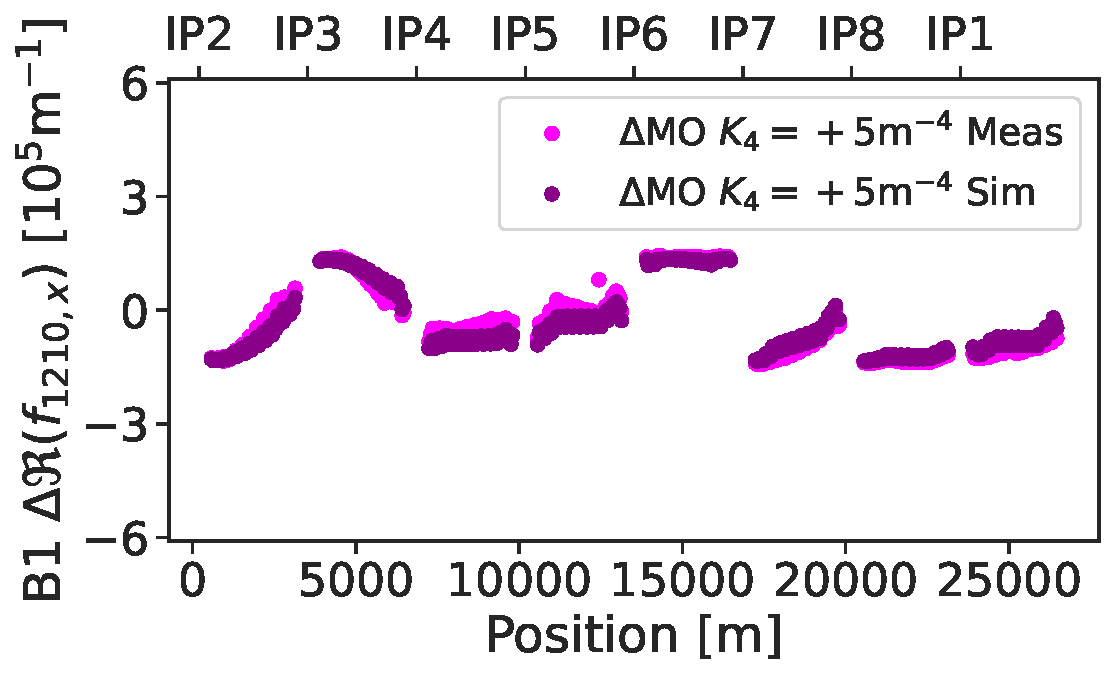
\includegraphics[width=\textwidth]{./images/skew_octupoles/responses_coupling/f1210_response_meas_sim_+5_REAL_smoll.pdf}
        %\caption{$f_{1210,x}$ for $K_4 = +5$}
    \end{subfigure}
    %
    \par\medskip 
    %
    \begin{subfigure}{0.47\textwidth}
        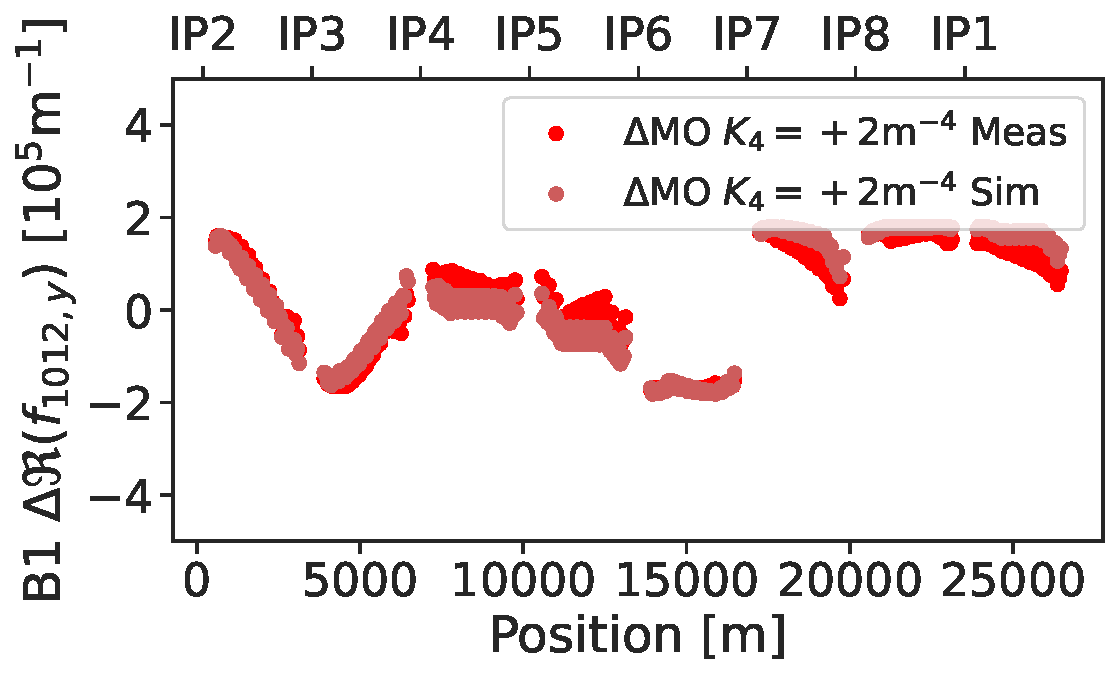
\includegraphics[width=\textwidth]{./images/skew_octupoles/responses_coupling/f1012_response_meas_sim_+2_REAL_smoll.pdf}
        %\caption{$f_{1012,y}$ for $K_4 = +2$}
    \end{subfigure}
    \hfill
    \begin{subfigure}{0.47\textwidth}
        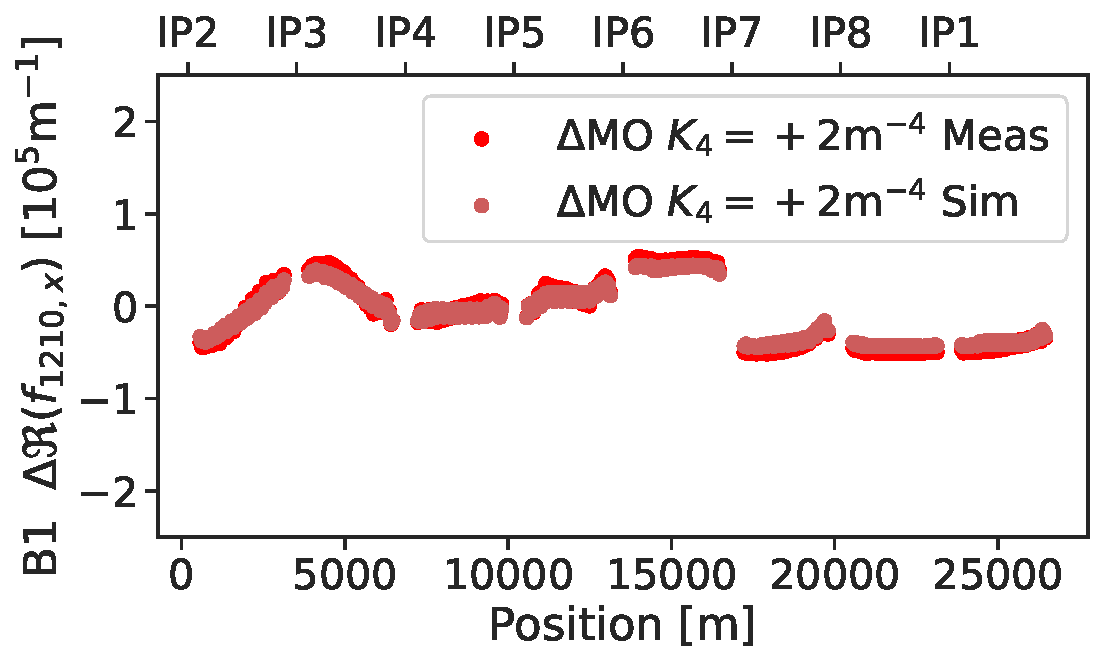
\includegraphics[width=\textwidth]{./images/skew_octupoles/responses_coupling/f1210_response_meas_sim_+2_REAL_smoll.pdf}
        %\caption{$f_{1210,x}$ for $K_4 = +2$}
    \end{subfigure}
    %
    \par\medskip 
    %
    \begin{subfigure}{0.47\textwidth}
        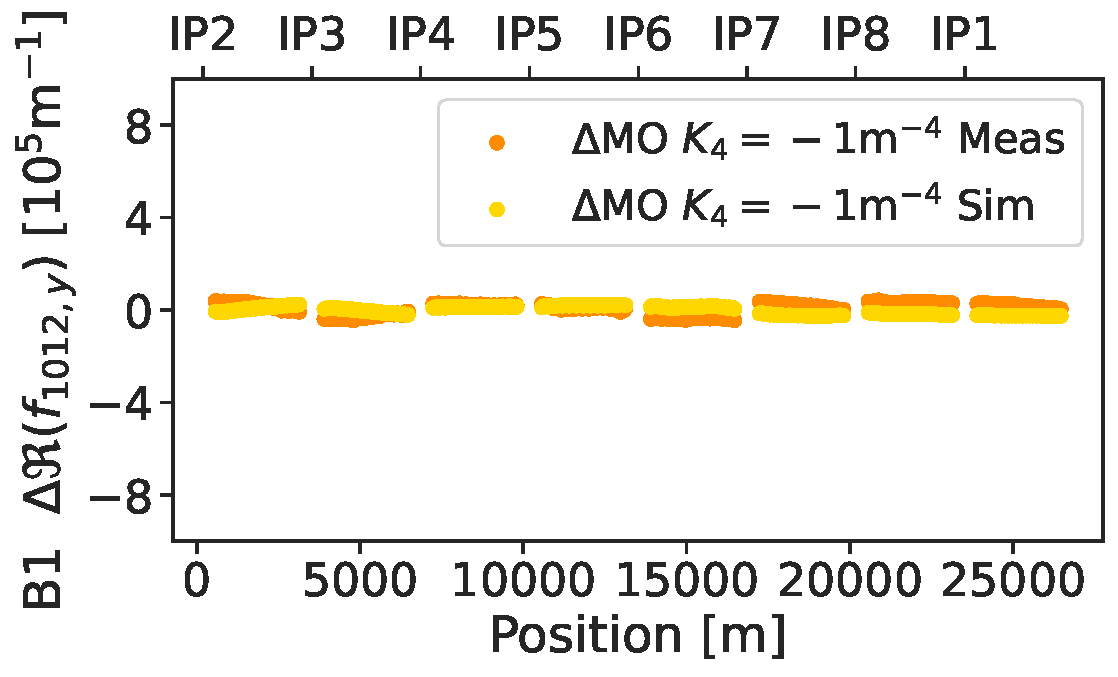
\includegraphics[width=\textwidth]{./images/skew_octupoles/responses_coupling/f1012_response_meas_sim_-1_REAL_smoll.pdf}
        %\caption{$f_{1012,y}$ for $K_4 = -1$}
    \end{subfigure}
    \hfill
    \begin{subfigure}{0.47\textwidth}
        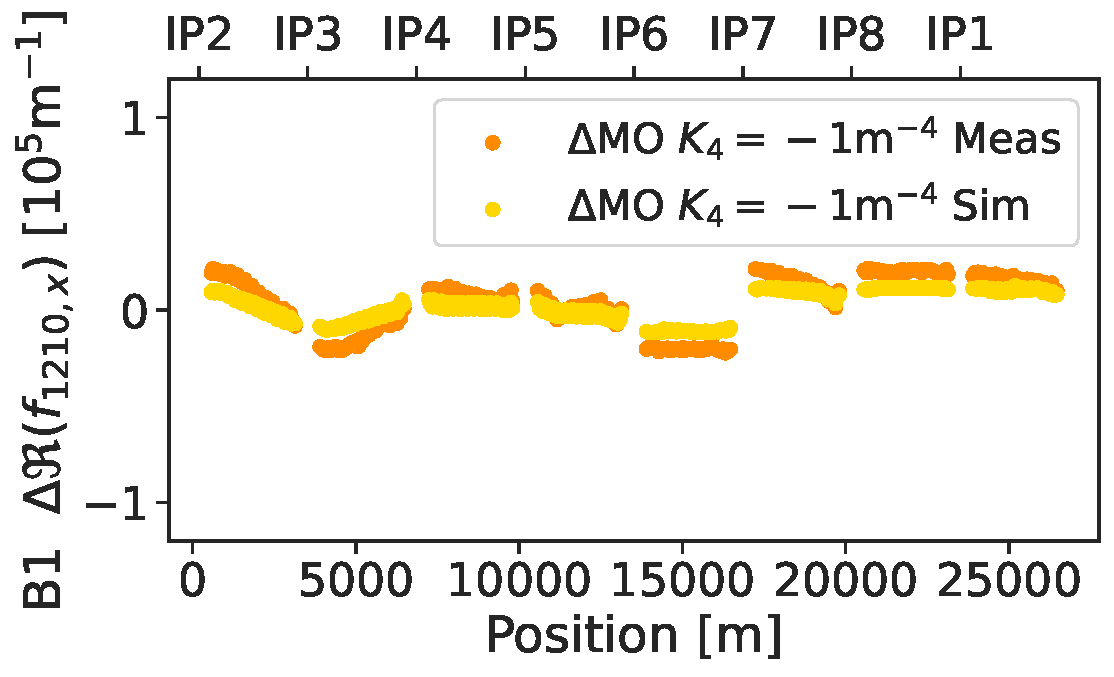
\includegraphics[width=\textwidth]{./images/skew_octupoles/responses_coupling/f1210_response_meas_sim_-1_REAL_smoll.pdf}
        %\caption{$f_{1210,x}$ for $K_4 = -1$}
    \end{subfigure}
    %
    \par\medskip
    %
    \begin{subfigure}{0.47\textwidth}
        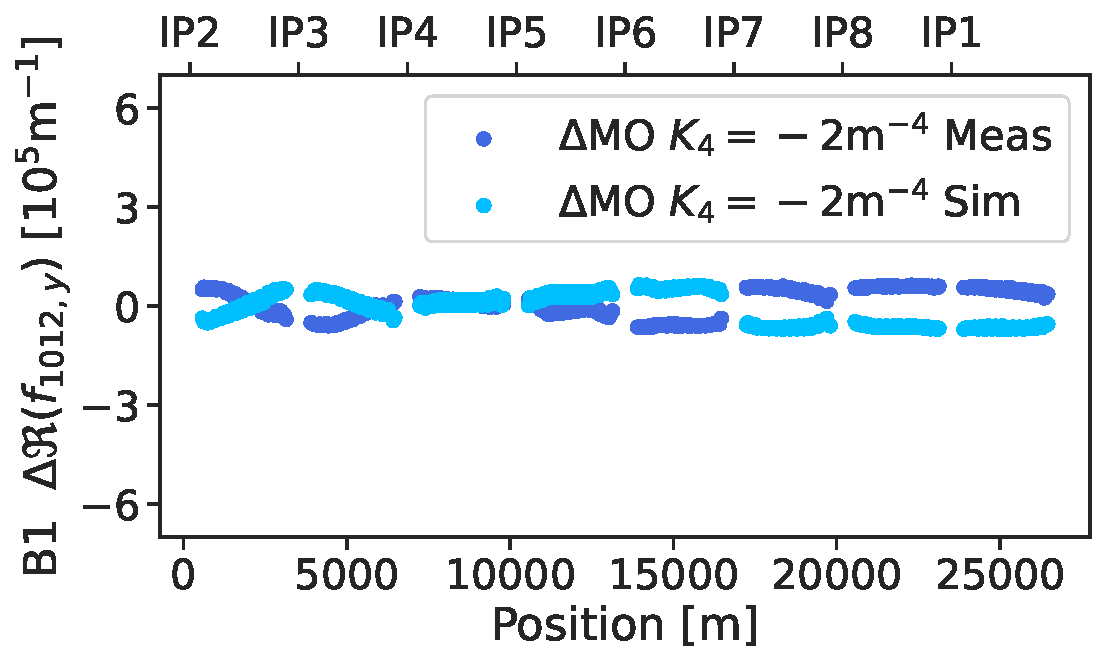
\includegraphics[width=\textwidth]{./images/skew_octupoles/responses_coupling/f1012_response_meas_sim_-2_REAL_smoll.pdf}
        %\caption{$f_{1012,y}$ for $K_4 = -2$}
    \end{subfigure}
    \hfill
    \begin{subfigure}{0.47\textwidth}
        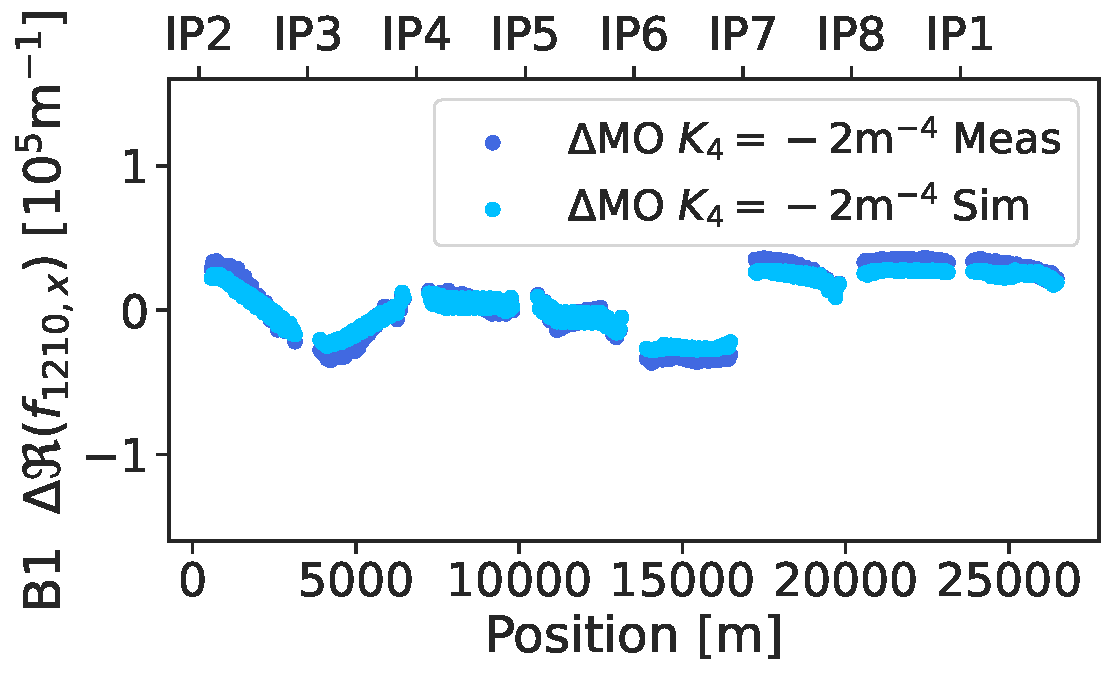
\includegraphics[width=\textwidth]{./images/skew_octupoles/responses_coupling/f1210_response_meas_sim_-2_REAL_smoll.pdf}
        %\caption{$f_{1210,x}$ for $K_4 = -2$}
    \end{subfigure}
    \caption{Measured and simulated real part shift of skew octupolar RDTs induced by Landau
    octupoles in presence of coupling at injection energy. Left column shows $f_{1012}$ while right
    shows $f_{1210}$.}
    \label{fig:skew_octupolar:response_meas_sim_coupling}
\end{figure}


% Imaginary Parts
%\begin{figure}[!htb]
%    \centering
%    \begin{subfigure}{0.47\textwidth}
%        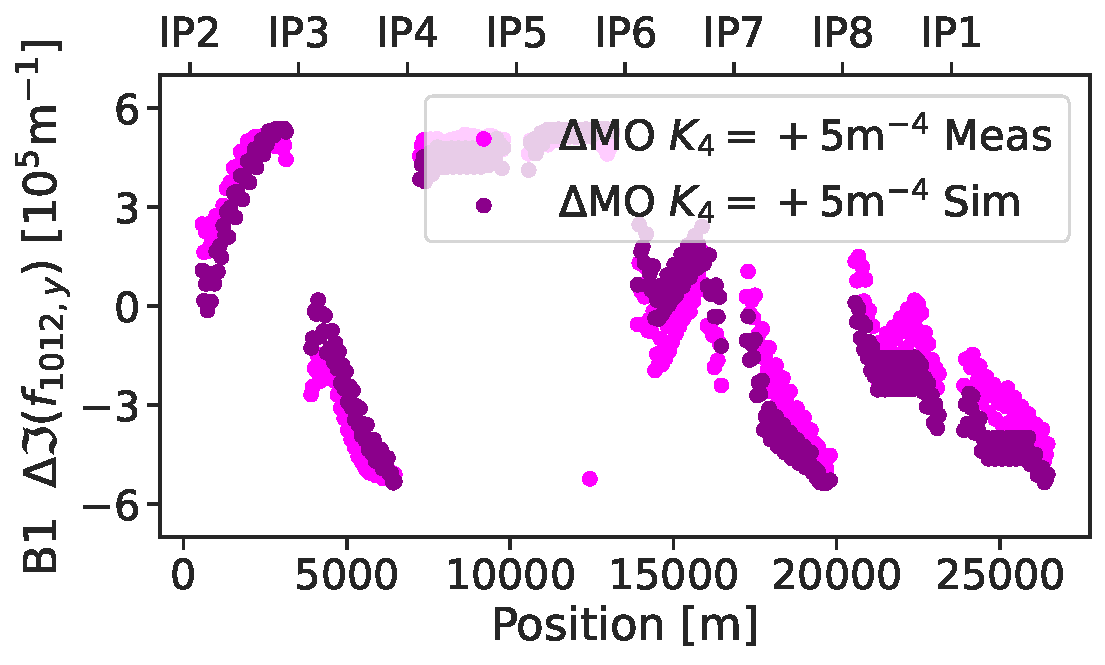
\includegraphics[width=\textwidth]{./images/skew_octupoles/responses_coupling/f1012_response_meas_sim_+5_IMAG_smoll.pdf}
%        %\caption{$f_{1012,y}$ for $K_4 = +5$}
%    \end{subfigure}
%    \hfill
%    \begin{subfigure}{0.47\textwidth}
%        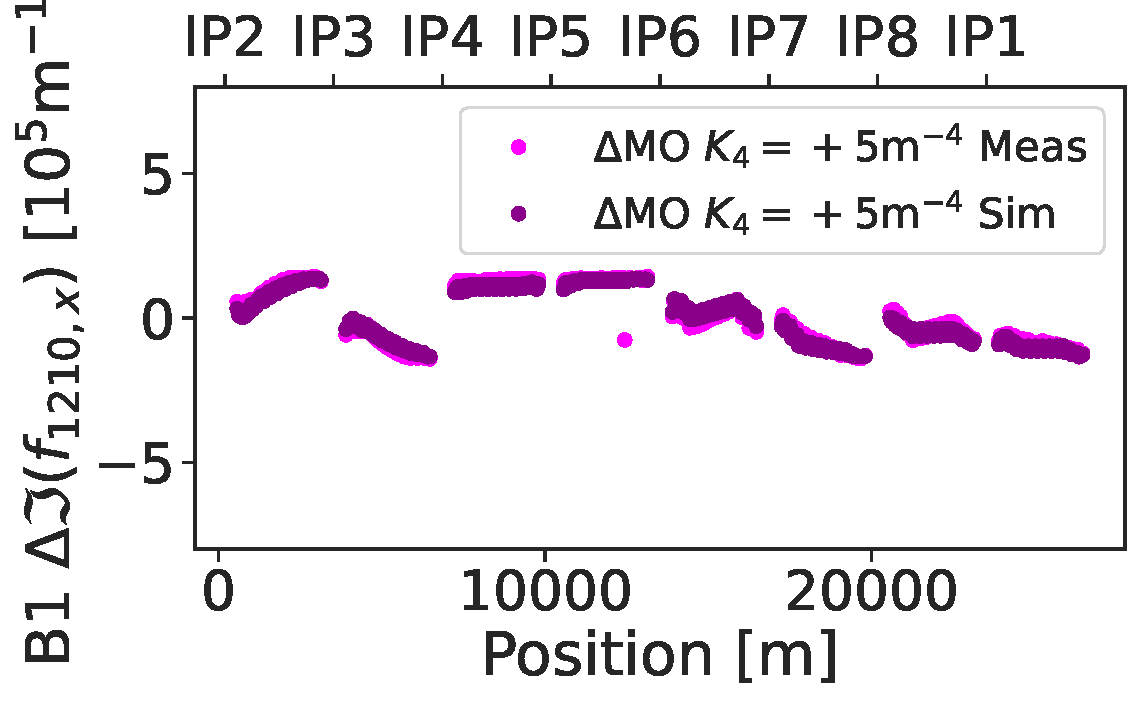
\includegraphics[width=\textwidth]{./images/skew_octupoles/responses_coupling/f1210_response_meas_sim_+5_IMAG_smoll.pdf}
%        %\caption{$f_{1210,x}$ for $K_4 = +5$}
%    \end{subfigure}
%    %
%    \par\medskip 
%    %
%    \begin{subfigure}{0.47\textwidth}
%        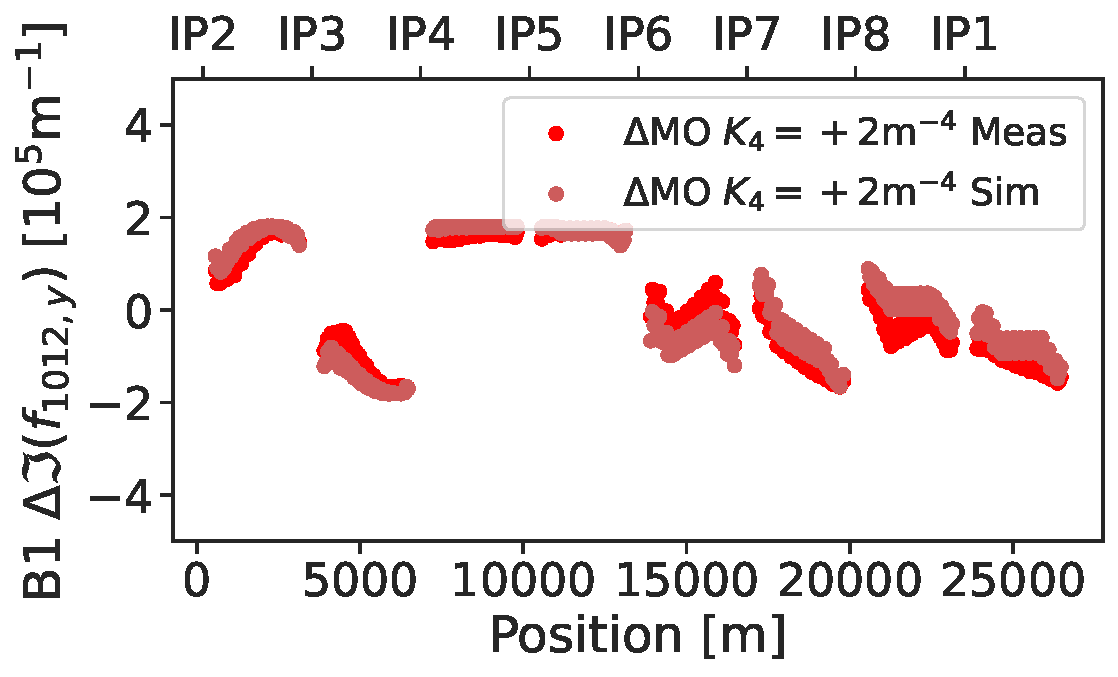
\includegraphics[width=\textwidth]{./images/skew_octupoles/responses_coupling/f1012_response_meas_sim_+2_IMAG_smoll.pdf}
%        %\caption{$f_{1012,y}$ for $K_4 = +2$}
%    \end{subfigure}
%    \hfill
%    \begin{subfigure}{0.47\textwidth}
%        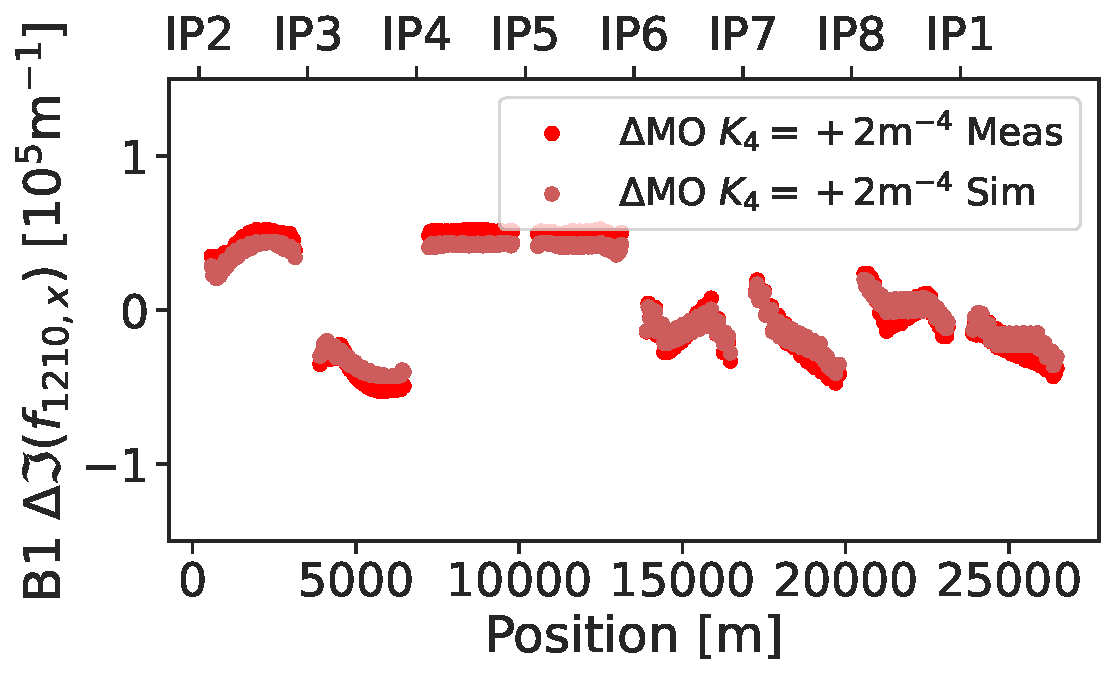
\includegraphics[width=\textwidth]{./images/skew_octupoles/responses_coupling/f1210_response_meas_sim_+2_IMAG_smoll.pdf}
%        %\caption{$f_{1210,x}$ for $K_4 = +2$}
%    \end{subfigure}
%    %
%    \par\medskip 
%    %
%    \begin{subfigure}{0.47\textwidth}
%        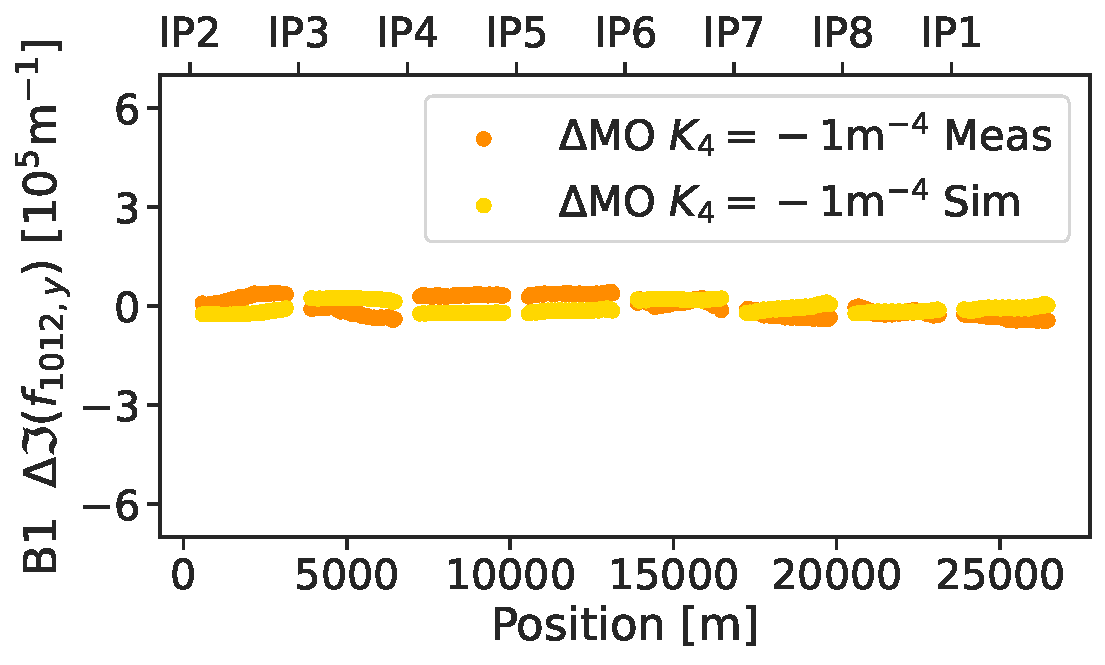
\includegraphics[width=\textwidth]{./images/skew_octupoles/responses_coupling/f1012_response_meas_sim_-1_IMAG_smoll.pdf}
%        %\caption{$f_{1012,y}$ for $K_4 = -1$}
%    \end{subfigure}
%    \hfill
%    \begin{subfigure}{0.47\textwidth}
%        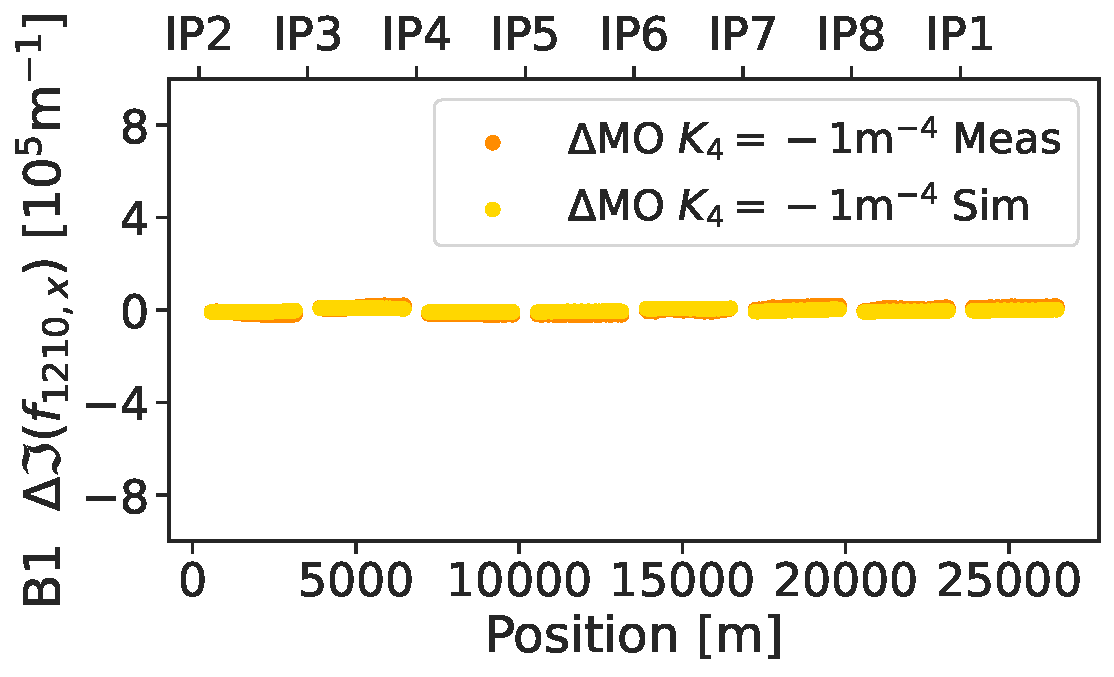
\includegraphics[width=\textwidth]{./images/skew_octupoles/responses_coupling/f1210_response_meas_sim_-1_IMAG_smoll.pdf}
%        %\caption{$f_{1210,x}$ for $K_4 = -1$}
%    \end{subfigure}
%    %
%    \par\medskip
%    %
%    \begin{subfigure}{0.47\textwidth}
%        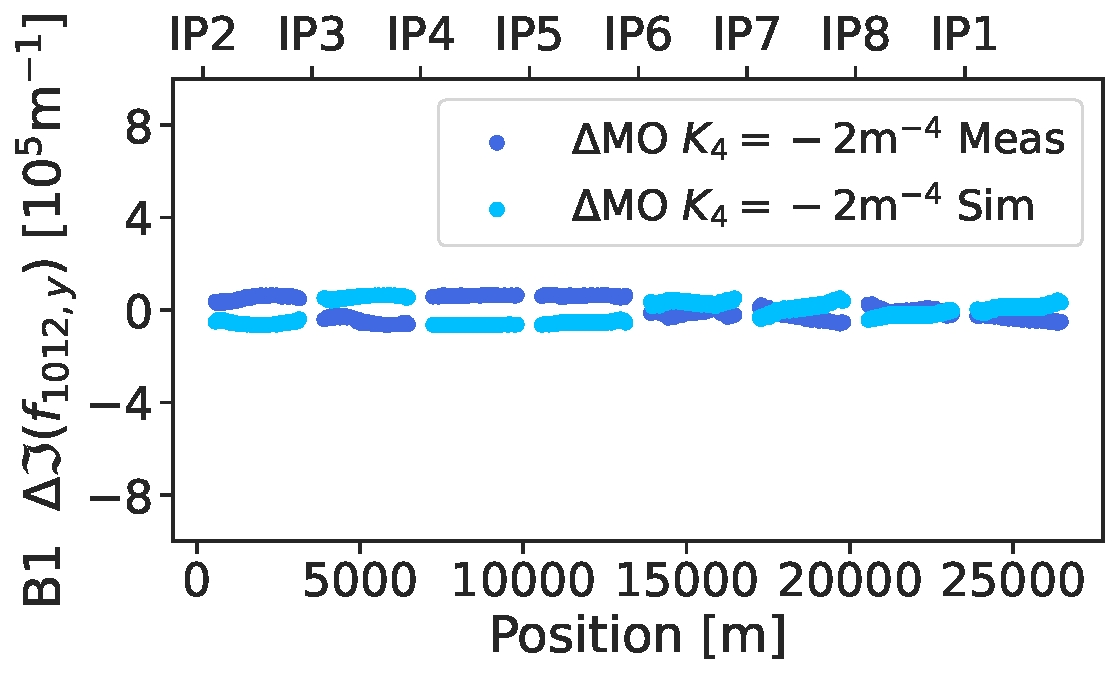
\includegraphics[width=\textwidth]{./images/skew_octupoles/responses_coupling/f1012_response_meas_sim_-2_IMAG_smoll.pdf}
%        %\caption{$f_{1012,y}$ for $K_4 = -2$}
%    \end{subfigure}
%    \hfill
%    \begin{subfigure}{0.47\textwidth}
%        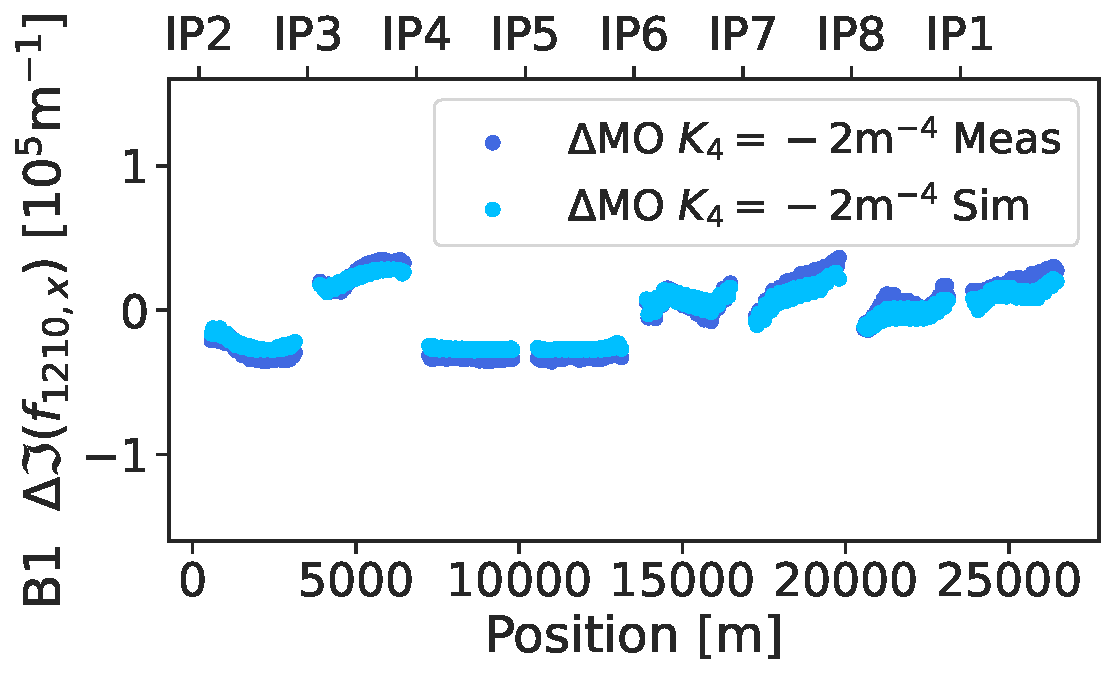
\includegraphics[width=\textwidth]{./images/skew_octupoles/responses_coupling/f1210_response_meas_sim_-2_IMAG_smoll.pdf}
%        %\caption{$f_{1210,x}$ for $K_4 = -2$}
%    \end{subfigure}
%    \caption{Measured and simulated imaginary part shift of skew octupolar RDTs induced by Landau
%    octupoles in presence of coupling at injection energy. Left column shows $f_{1012}$ while right
%    shows $f_{1210}$.}
%    \label{fig:skew_octupolar:response_meas_sim_coupling_imag}
%\end{figure}

As demonstrated in \cref{fig:skew_octupolar:sim_coupling}, Landau octupoles, along with minor
variations in coupling, even at low $K_4$ strengths, can significantly influence the RDTs
$f_{1012}$ and $f_{1210}$, along with their associated resonances. Furthermore, at their
operational powering of $K_4=18$, Landau octupoles are anticipated to generate very large skew
octupolar RDTs, as simulated in \cref{fig:skew_octupolar:mo_full_power_coupling_simulation}, where a
realistic operational coupling value is utilized. A difference of two orders of magnitude is
observed when powering the octupoles and considering coupling.
Such a drastic worsening of the RDTs could prompt for further studies and corrections.

\begin{figure}[!htb]
    \centering
    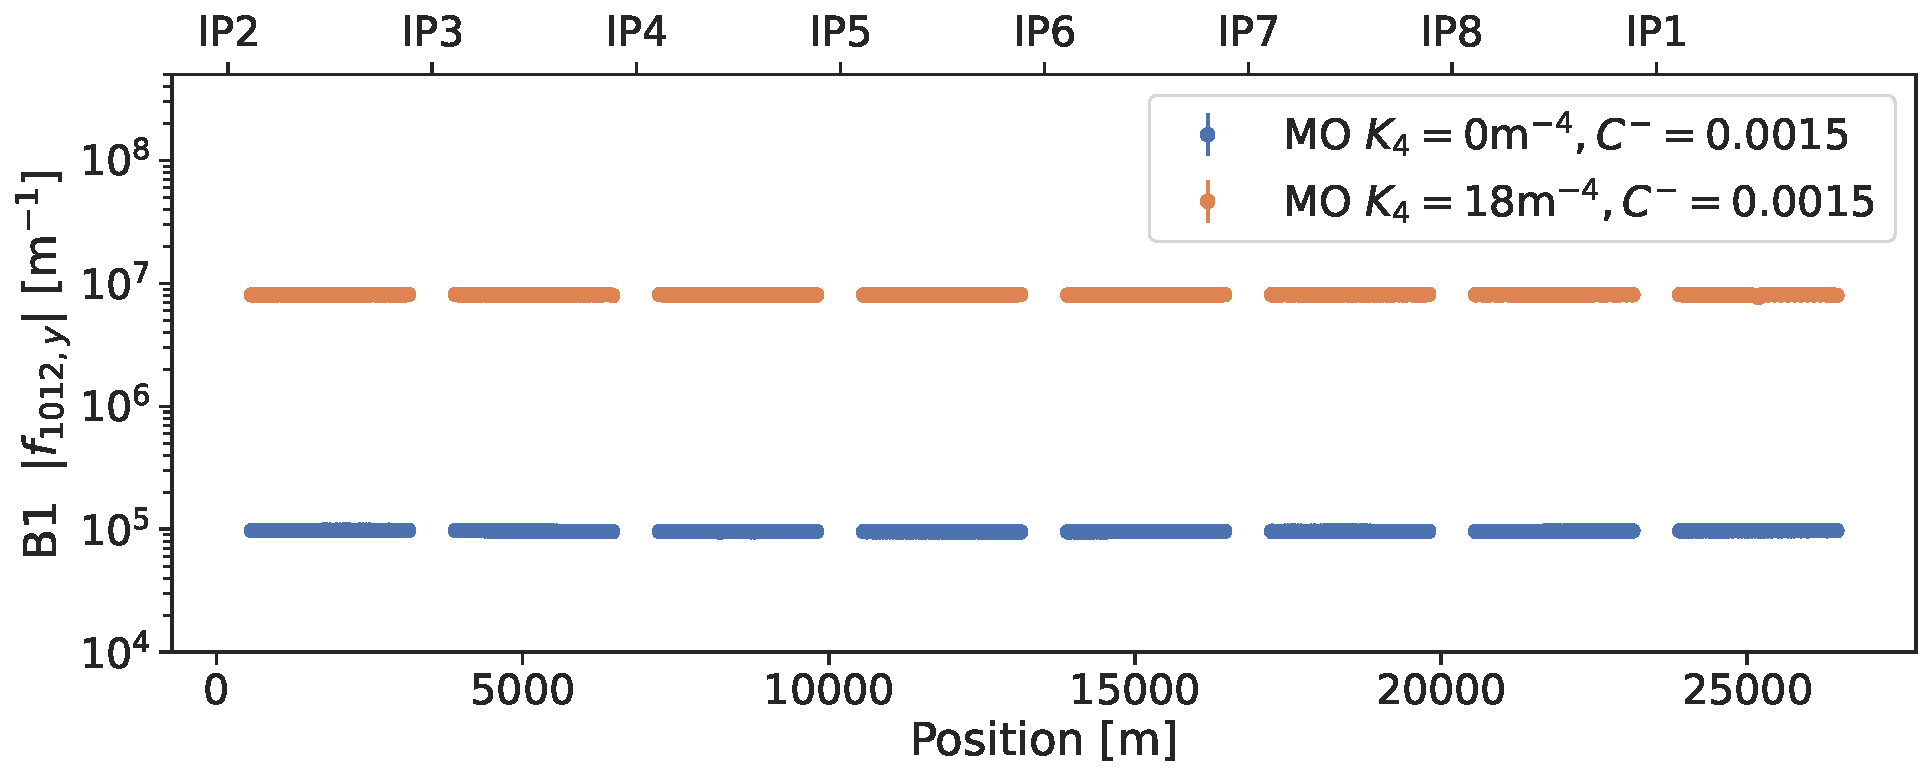
\includegraphics[width=0.8\textwidth]{./images/skew_octupoles/f1012_AMP_full_mo_with_coupling.pdf}
    \caption{Simulated skew octupolar RDT $f_{1012}$ with Landau octupoles turned off and at their
    operational powering. Coupling is set to a value commonly seen in operation for both.}
    \label{fig:skew_octupolar:mo_full_power_coupling_simulation}
\end{figure}


%=============================
%        Conclusion
%=============================
\FloatBarrier
\section{\review{Summary}}

This chapter investigates the origins of skew-octupolar fields in the LHC and explores methods for
measuring and mitigating their effects. The studies demonstrate that these fields significantly
contribute to limitations in dynamic aperture, particularly when the beam is kicked with the
AC-Dipole. 

For the first time, skew-octupolar Resonance Driving Terms have been directly corrected using
a response matrix-based approach at top energy. This new method facilitates a more efficient use of
dedicated machine time compared to previous empirical approaches. The corrections successfully
correct the RDTS $f_{1012}$ and $f_{1210}$

Furthermore, the chapter addresses the unexpected influence of Landau octupoles on skew-octupolar
RDTs at injection energy. Simulations reveal that misalignments of the Landau octupoles,
particularly roll errors, do not have a significant impact. Instead, transverse linear coupling
emerges as a crucial factor.
Initial findings indeed suggest that coupling is essential for predicting the behavior of
skew-octupolar RDTs in the presence of Landau octupoles. During regular operation, where the Landau
octupoles are powered at $K_4 = 18$, significant skew-octupolar RDTs are expected to be generated
and degrade the dynamic aperture.

The results presented provide valuable insights into the complex interplay of magnetic fields in the
LHC and underscore the importance of accurate modeling for effective corrections. Moreover, the
implemented corrections have substantially improved the forced dynamic aperture, enabling the
high-amplitude kicks necessary for non-linear optics measurements. These corrections can also be
computed online in the control room, thereby reducing commissioning time and increasing the
integrated luminosity of the LHC.
